% ABOUTME: Main document of the Phase 1 IEEE conference report for team T081.
% ABOUTME: Title, authors and abstract; every section is a fragment under sections/.
\documentclass[conference]{IEEEtran}
\usepackage{graphicx}
\usepackage{amsmath}
\usepackage{cite}

\begin{document}

\title{Remaining Useful Life Prediction on NASA C-MAPSS FD001 with Engineered Degradation Features}

\author{\IEEEauthorblockN{Sarvesh Srinath, Trishit Swarnakar, Aryan Kumar,
Husain Khorakiwala and Navodit Sharma}
\IEEEauthorblockA{Team T081, Section E, CSAI Project 7}}

\maketitle

\begin{abstract}
We predict the remaining useful life (RUL) of turbofan engines in the FD001
subset of NASA C-MAPSS from their multivariate sensor histories. Rolling
means, standard deviations and least squares slopes over windows of 5, 10
and 20 cycles, together with a learned health index, are computed within
each engine. Elastic Net, Random Forest and XGBoost are tuned with
five-fold cross validation grouped by engine on RUL capped at 125 cycles,
and the 100 test engines are scored once, at their last observed cycle,
after every choice is frozen. The selected XGBoost model reaches a test
RMSE of 15.36 cycles and a late-stage RMSE of 7.03 cycles on engines within
50 cycles of failure. Against test labels clipped at 125, Random Forest and
XGBoost reach RMSE 14.02 and 14.08, improving on published Random Forest
and gradient boosting results and trailing the best published deep models
by 0.8 to 1.4 cycles. Most of the gain over raw sensors comes from the
engineered features rather than the choice of learner.
\end{abstract}

\begin{IEEEkeywords}
remaining useful life, prognostics, C-MAPSS, feature engineering, gradient
boosting, random forest, SHAP
\end{IEEEkeywords}

% ABOUTME: Introduction section of the IEEE report.
% ABOUTME: Motivation for RUL prediction, the C-MAPSS benchmark, our approach, contributions and paper layout.
\section{Introduction}
\label{sec:intro}

Maintenance of aircraft engines is either scheduled at fixed intervals or
triggered by observed condition. Fixed intervals replace parts that still
have life left, while waiting for a fault risks a failure in service.
Predicting the remaining useful life (RUL) of an engine, the number of
operating cycles left before it fails, lets maintenance be planned close to
the point where it is actually needed. The cost of an error is asymmetric:
predicting too much remaining life risks an in-service failure, while
predicting too little only brings maintenance forward.

The NASA Commercial Modular Aero-Propulsion System Simulation (C-MAPSS)
data~\cite{saxena2008damage} are the standard public benchmark for this
task. Each engine is simulated from a healthy state with unknown initial
wear, and 21 sensors and three operating settings are recorded once per
cycle. Training engines run to failure; test engines are cut off at an
unknown point, and the true RUL is given only at their last observed cycle.
We work on the FD001 subset, which has one operating condition and one
fault mode.

Our approach keeps the learners simple and puts the effort into the
features and the protocol. From the 14 sensors that vary in FD001 we
compute, within each engine, rolling means, standard deviations and least
squares slopes over three window lengths, and a health index learned by
linear regression. Elastic Net, Random Forest and XGBoost are trained on
RUL capped at 125 cycles and tuned with five-fold cross validation grouped
by engine, so that no engine contributes rows to both sides of a split. The
test set is used once, after every hyperparameter and the choice of model
are frozen.

The contributions of this report are:
\begin{itemize}
\item an engine-level evaluation protocol for FD001 in which feature
statistics are refitted inside every fold and the test set is scored once,
with errors reported separately for engines near failure;
\item a comparison of three regressors on raw and engineered features,
showing that the engineered features improve every model and account for
most of the gain over raw sensors;
\item an analysis of what the tree ensembles rely on, using held-out
grouped permutation importance and SHAP values, and a comparison of the
test results with published FD001 models under matched label clipping.
\end{itemize}

Section~\ref{sec:related} reviews prior work on C-MAPSS.
Section~\ref{sec:data} describes the data and the choice of sensors and
target cap, and Section~\ref{sec:evaluation} the evaluation protocol.
Section~\ref{sec:features} defines the engineered features.
Section~\ref{sec:models} covers the models, their tuning and what they rely
on, and Section~\ref{sec:results} reports the test results.
Section~\ref{sec:discussion} discusses the findings and their limits, and
Section~\ref{sec:conclusion} concludes with the plan for sequence models.

% ABOUTME: Related work section of the IEEE report (issue #8).
% ABOUTME: C-MAPSS, the capped RUL target, classical and deep FD001 models, and the gap tested here.
\section{Related Work}
\label{sec:related}

\subsection{Benchmark and target}
C-MAPSS simulates run-to-failure trajectories of aircraft turbofan engines
with modelled damage propagation~\cite{saxena2008damage}. Its FD001
subset is the simplest of the four: one operating condition, one fault mode
(high-pressure compressor degradation), and 100 training and 100 test
engines. Training engines run until failure; each test engine stops at an
unknown point before failure and its true RUL at that cycle is given
separately.

A linear RUL target implies that an engine degrades at a constant rate from
its first cycle, which the sensors do not show. Heimes~\cite{heimes2008rnn},
who estimated RUL with recurrent neural networks, proposed the
piecewise-linear target used in much of the later
work~\cite{babu2016cnn,ragab2020attention}: the target is held at a
constant maximum early in life and falls linearly to zero at failure. The
maximum is chosen from the data and differs between
subsets~\cite{babu2016cnn}; Ragab et al.\ use 125 cycles for FD001 and
FD003 and 130 for FD002 and FD004~\cite{ragab2020attention}. We cap
training targets at 125.

\subsection{Classical models}
Early data-driven methods for this benchmark include similarity-based
prognostics~\cite{wang2008similarity}. In the experiments of Babu et
al.~\cite{babu2016cnn}, support vector regression reached an RMSE of 20.96
cycles on FD001, ahead of relevance vector regression (23.80) and a
multilayer perceptron (37.56). Zhang et al.~\cite{zhang2017modbne} report
17.91 for a Random Forest and 15.67 for gradient boosting, against 15.04
for their ensemble of deep belief networks. These tree ensembles are the
closest published counterparts of our models.

\subsection{Deep sequence models}
Deep models take a window of normalised sensor readings as input and learn
their own features. Babu et al.~\cite{babu2016cnn} applied a convolutional
network along the time axis of 15-cycle windows (RMSE 18.45). Zheng et
al.~\cite{zheng2017lstm} used a long short-term memory
(LSTM)~\cite{hochreiter1997lstm} network, whose gated memory cells can carry
information over long time lags (16.14). Li et al.~\cite{li2018dcnn}
used a one-dimensional CNN with multiple input channels; at 12.61 it has
the lowest FD001 RMSE in the comparison of Ragab et
al.~\cite{ragab2020attention}. Ragab et al.\ add an attention mechanism
to an LSTM encoder-decoder over 30-cycle windows of 14 sensors and reach
12.63, with the lowest score $S$ (Section~\ref{sec:evaluation}) in that
comparison. Table~\ref{tab:related} summarises these methods;
Table~\ref{tab:published} in Section~\ref{sec:results} places our test
results among them.

\begin{table}[t]
\centering
\caption{Representative FD001 methods. RMSE values are those collected
in~\cite{ragab2020attention}, Table III, except SVR, which is
from~\cite{babu2016cnn}. Ours is scored against test labels clipped at 125,
as in Table~\ref{tab:published}. Cap is the maximum of the training
target. A dash marks a setting not stated in~\cite{babu2016cnn}
or~\cite{ragab2020attention}.}
\label{tab:related}
\footnotesize
\begin{tabular}{llrl}
\hline
Method & Input & RMSE & Cap \\
\hline
SVR \cite{babu2016cnn}                 & --                    & 20.96 & -- \\
Random Forest \cite{zhang2017modbne}   & --                    & 17.91 & -- \\
Grad.\ boosting \cite{zhang2017modbne} & --                    & 15.67 & -- \\
2D CNN \cite{babu2016cnn}              & sensors, 15 cycles    & 18.45 & yes \\
Deep LSTM \cite{zheng2017lstm}         & sensor sequence       & 16.14 & -- \\
1D CNN \cite{li2018dcnn}               & sensor windows        & 12.61 & -- \\
ATS2S \cite{ragab2020attention}        & 14 sensors, 30 cycles & 12.63 & 125 \\
XGBoost (ours)                         & engineered            & 14.08 & 125 \\
\hline
\end{tabular}
\end{table}

\subsection{Gap addressed}
The most accurate FD001 results come from models that learn features from
raw sensor windows. This work asks how far hand-built degradation features
take classical models. For each of the 14 informative sensors we compute
the rolling mean, standard deviation and least squares slope over 5, 10
and 20 cycles, after operating regime normalisation, and keep the
normalised readings, the cycle number and a regression-based health index
(Section~\ref{sec:features}). Elastic Net, Random Forest and XGBoost are
trained on these features and tuned with cross validation grouped by
engine, so that no engine appears in both the training and validation
folds and the validation error is not inflated by near-duplicate cycles
(Section~\ref{sec:evaluation}). Sequence models of the kind discussed
above are the subject of the second phase of the project.

% ABOUTME: Dataset quality, sensor selection and RUL target rationale for FD001.
% ABOUTME: Training decisions and final descriptive test evidence produced by notebooks/01_eda.ipynb (issue #3).
\section{Dataset and Exploratory Analysis}
\label{sec:data}

\subsection{Dataset and quality checks}
We use the FD001 subset of NASA C-MAPSS, a simulated turbofan degradation
benchmark with one nominal operating condition and one fault mode: high-pressure
compressor degradation~\cite{saxena2008damage}. Each observation contains an
engine identifier, a cycle number, three operating settings and 21 sensor readings.
The training set contains 20,631 observations from 100 engines run to failure.
All sensor and target decisions use this training set. A final subsection adds
descriptive test plots approved in review; no earlier choice was revisited.

We found no missing cells, duplicate rows or duplicate engine-cycle keys.
Cycles start at one and are consecutive within each engine, so no imputation
or row removal was needed. Recorded lifetimes range from 128 to 362 cycles,
with median 199 and mean 206.31 cycles. Figure~\ref{fig:eda-lifetimes} shows
the distribution of lifetimes, counting each engine once, and the RUL
distribution, counting every cycle. The latter weights longer histories more
heavily. These descriptive distributions are not model evaluation results.

\begin{figure*}[t]
  \centering
  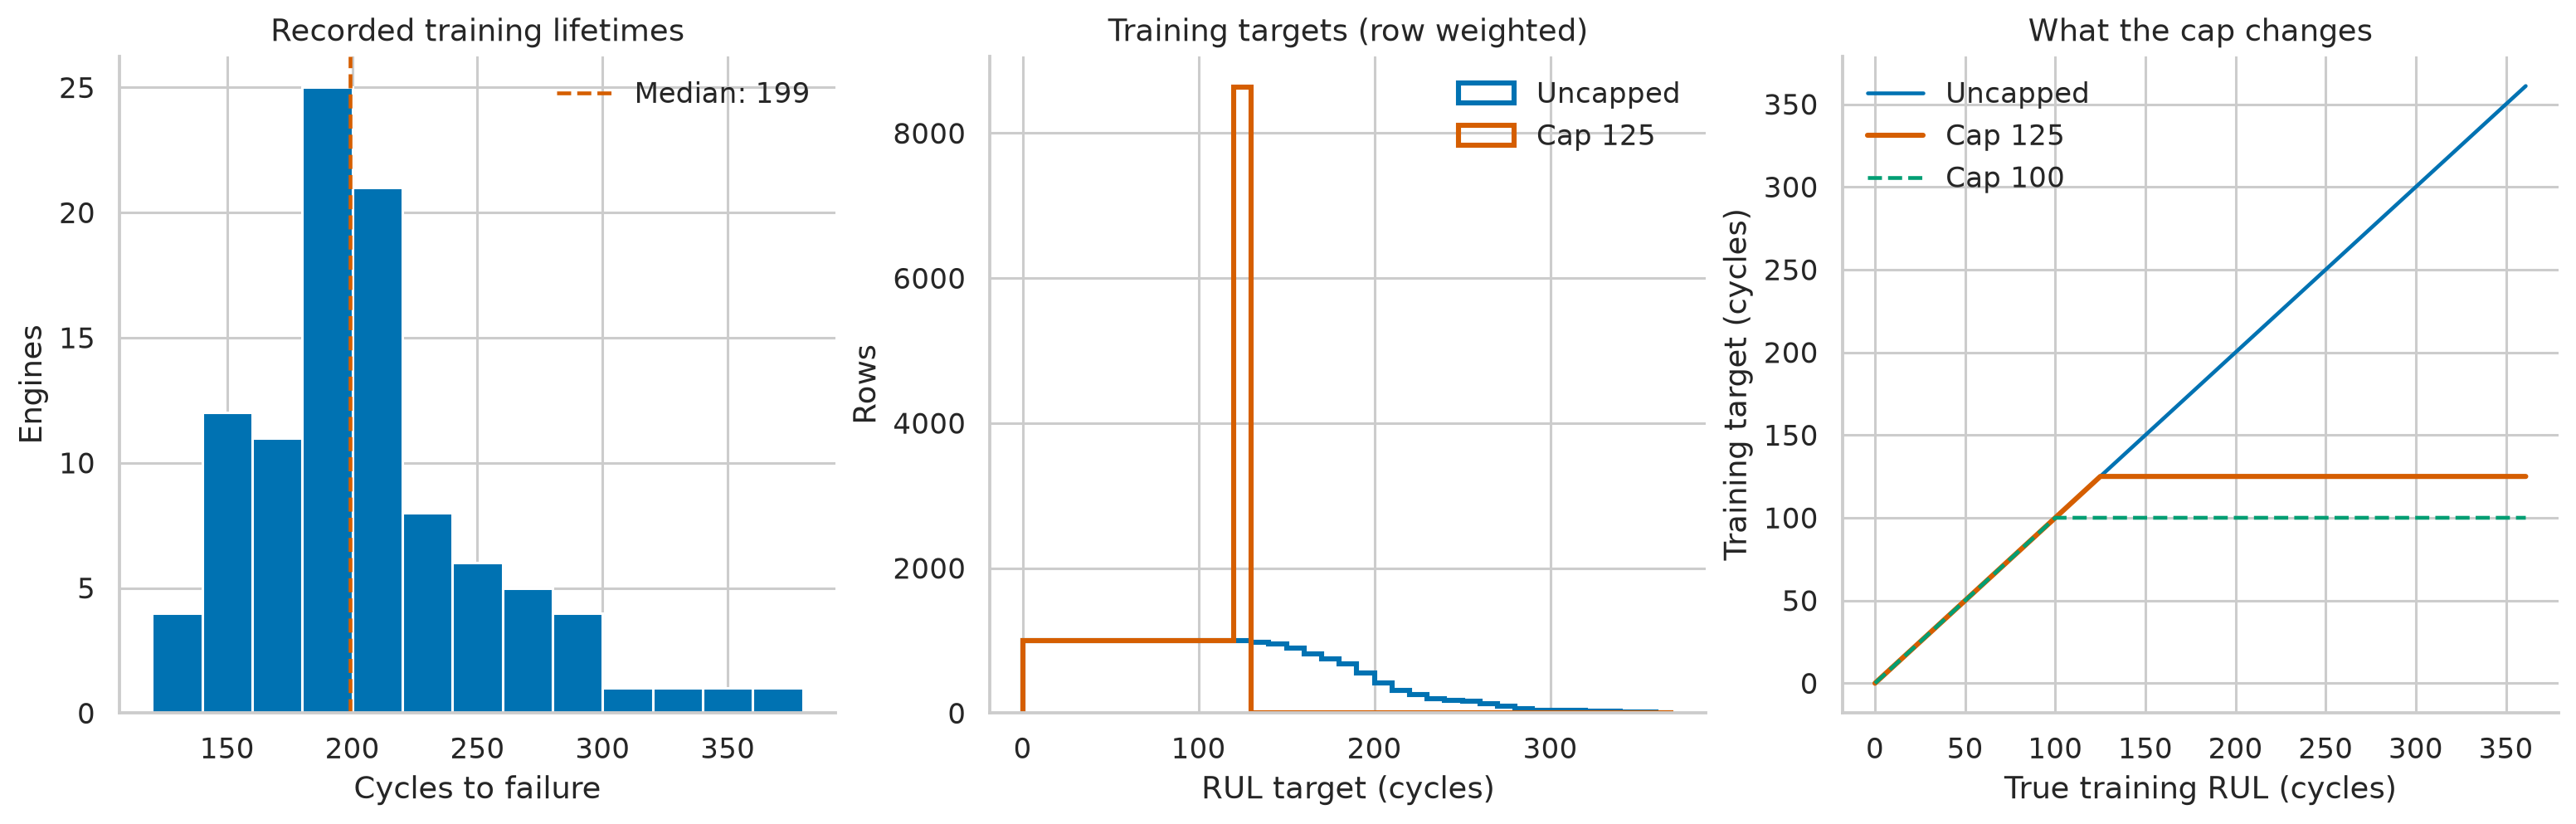
\includegraphics[width=\textwidth]{../figures/eda_lifetimes_rul.png}
  \caption{Training lifetimes, uncapped and capped training targets, and the
  effect of caps of 100 and 125 cycles. The cap changes labels, not the number
  of observations.}
  \label{fig:eda-lifetimes}
\end{figure*}

\subsection{Operating settings and sensor selection}
Settings 1 and 2 vary slightly around zero, while setting 3 is exactly 100.
The scatter plots in Fig.~\ref{fig:eda-settings} are consistent with the
single nominal operating condition specified by NASA. A noisy cloud alone
does not establish a physical regime count; no regime clustering is fit here.

\begin{figure}[t]
  \centering
  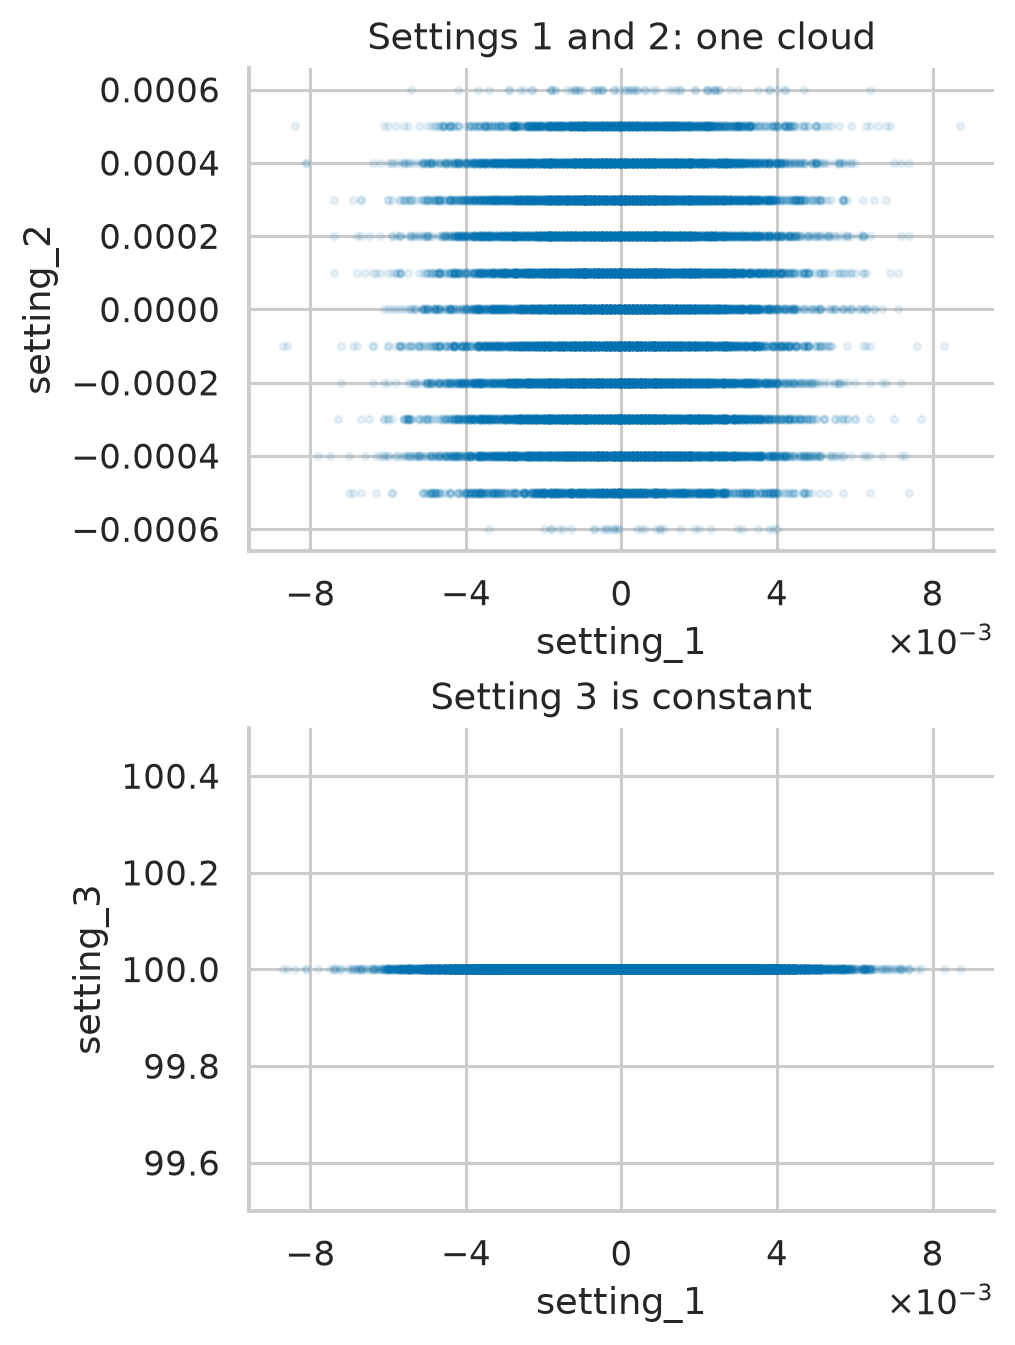
\includegraphics[width=\columnwidth]{../figures/eda_operating_settings.png}
  \caption{Training operating settings: a cloud around zero for settings 1
  and 2, and a constant value for setting 3.}
  \label{fig:eda-settings}
\end{figure}

We compute sample standard deviation, range, distinct-value count and
dominant-value fraction for each sensor. Raw standard deviations are in
different physical units, so an absolute variance threshold would not give
a fair comparison. Sensors $s_1,s_5,s_{10},s_{16},s_{18},s_{19}$ each have
one unique reading and are removed as exact constants. Tiny nonzero
standard deviations for some constants are floating-point roundoff.

We also remove $s_6$, whose only recorded levels are 21.60 and 21.61,
consistent with quantization or rounding at the recorded precision. Its standard
deviation is approximately 0.001389: 20,225 readings are 21.61 and 406 are 21.60.
The 98.03\% dominant share is descriptive, not a selection threshold.
This FD001 choice matches the 14-sensor set listed by Liu et al.~\cite{liu2021rul},
Section 4.2; it does not prove zero predictive information.
The resulting 14 retained sensors are
$s_2,s_3,s_4,s_7,s_8,s_9,s_{11},s_{12},s_{13},s_{14},s_{15},s_{17},s_{20},s_{21}$.
Sensor $s_{17}$ is quantized but has 13 distinct readings and is retained.
Figure~\ref{fig:eda-sensors} summarizes this evidence; the same list is
exported as \texttt{USEFUL\_SENSORS} for feature engineering.

\begin{figure}[t]
  \centering
  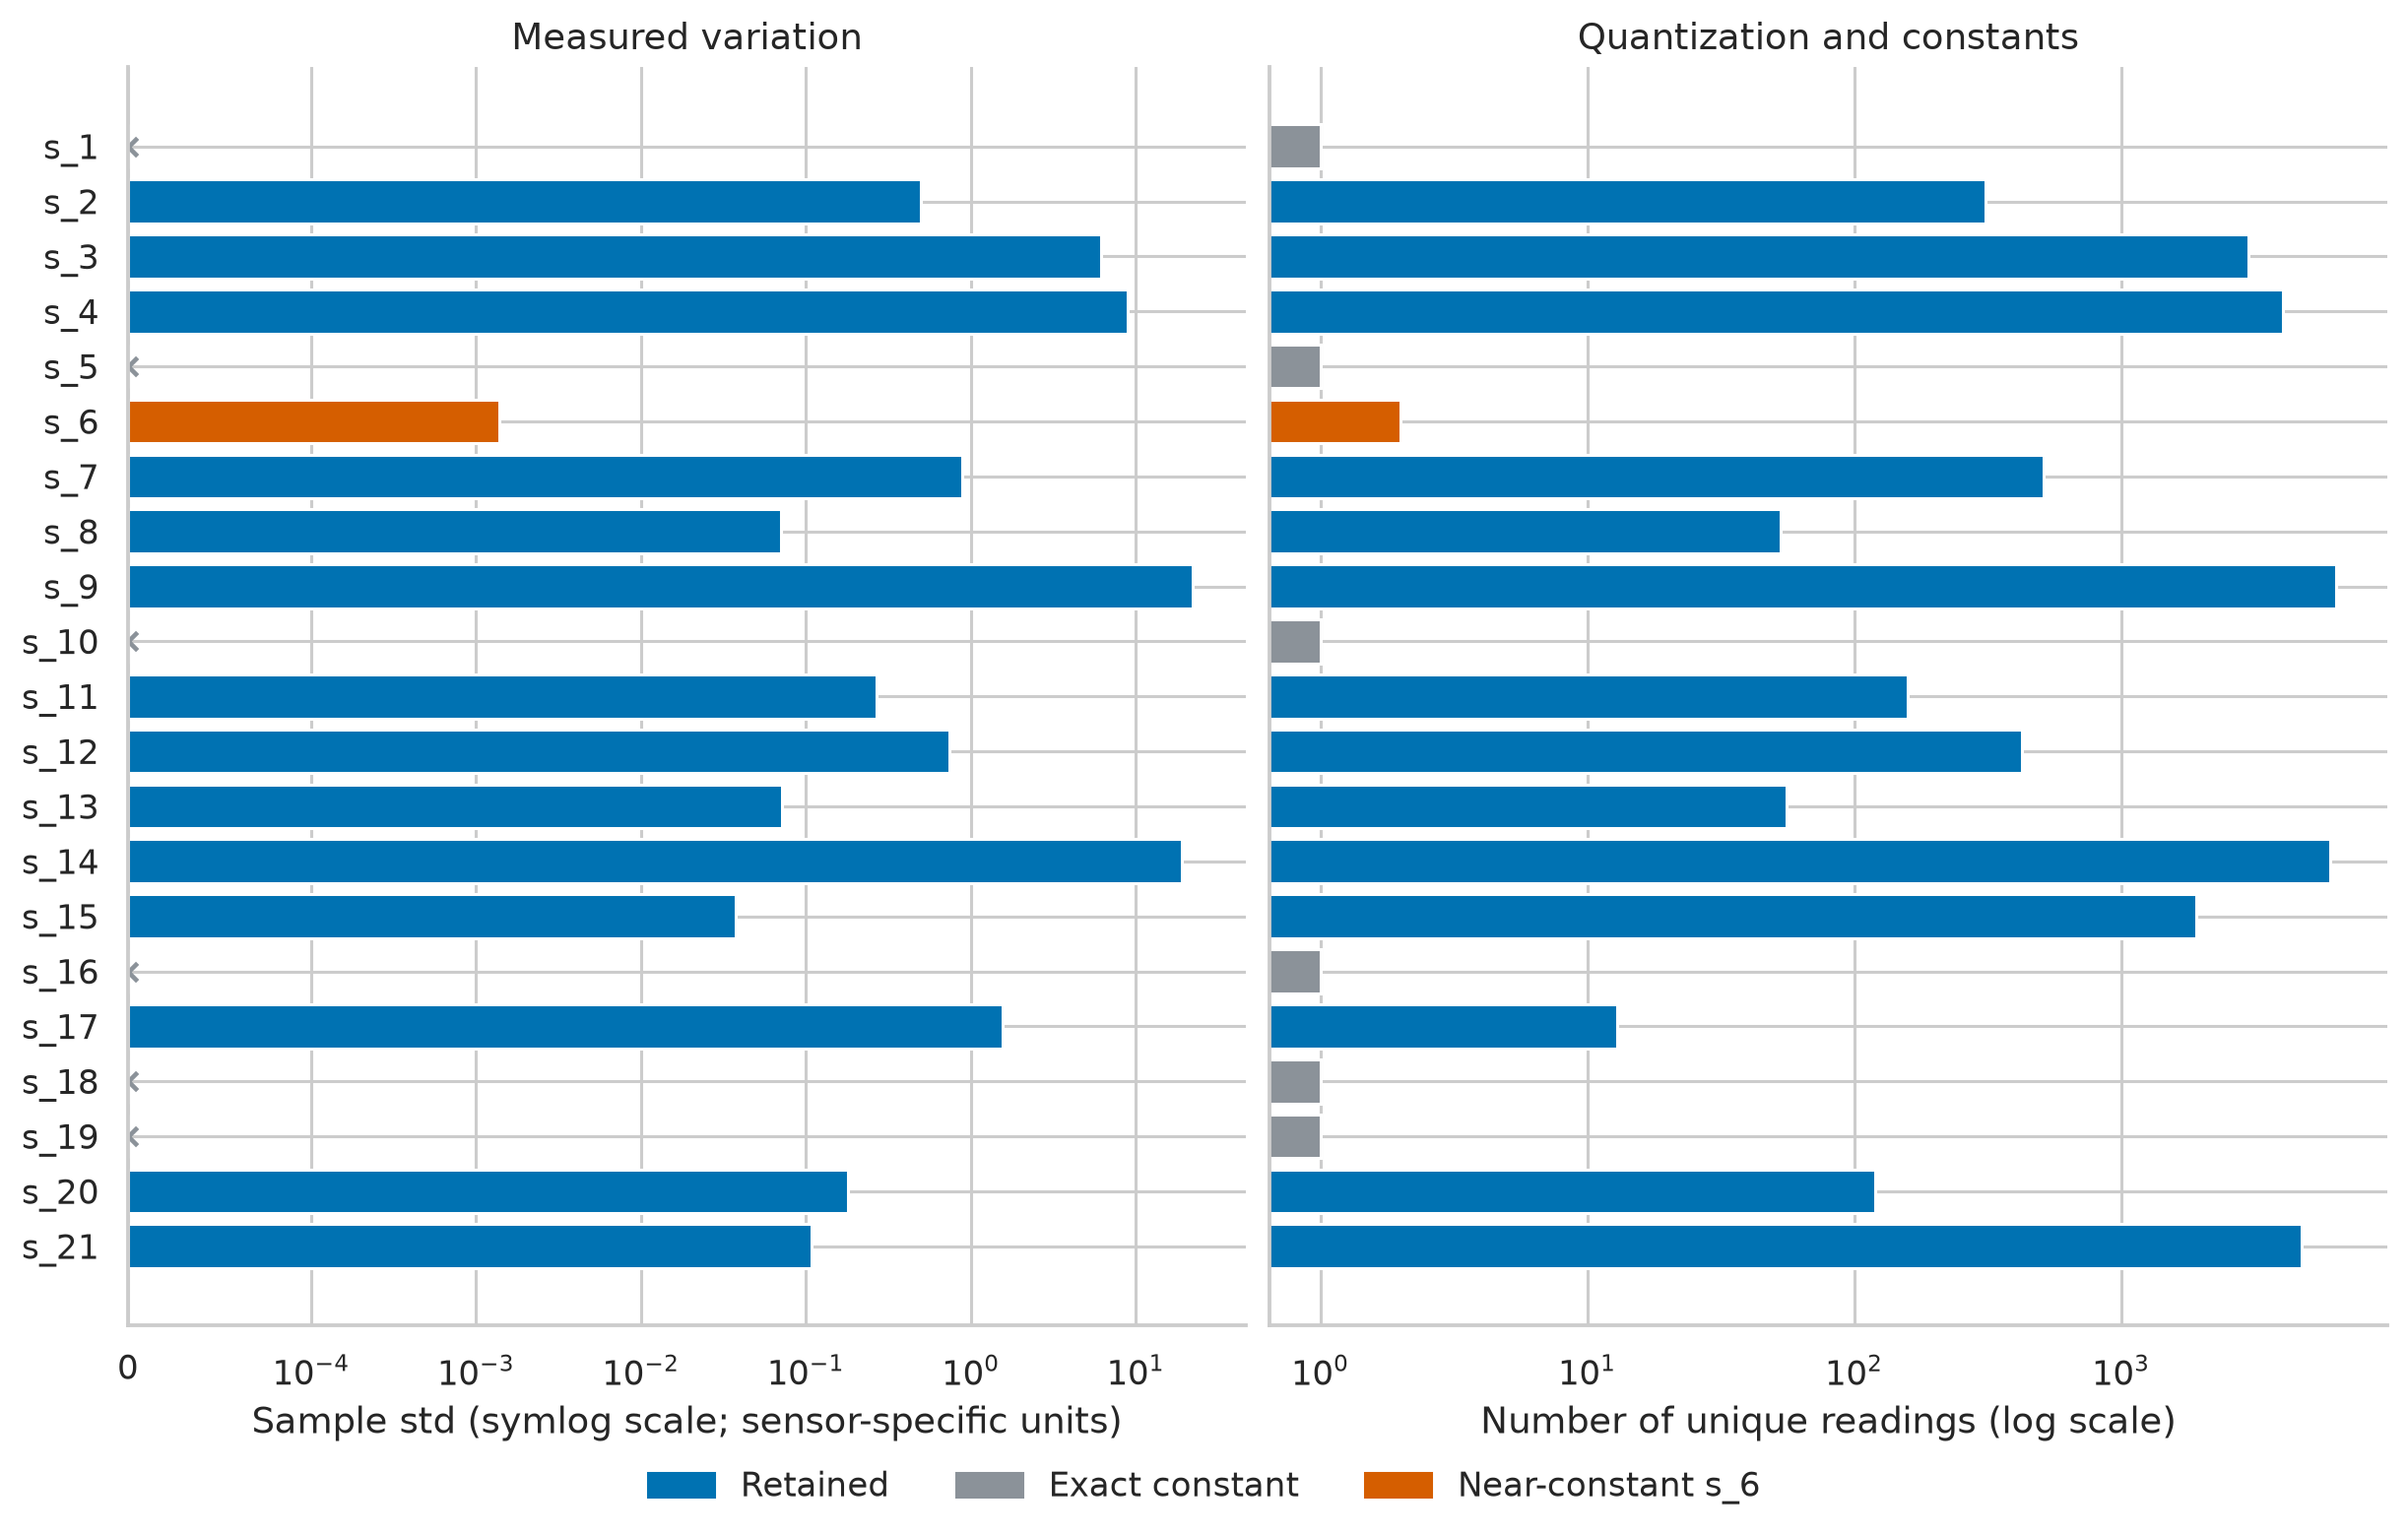
\includegraphics[width=\columnwidth]{../figures/eda_sensor_variation.png}
  \caption{Sensor variation and distinct-value counts. Exact constants are
  shown at zero standard deviation; sensor units differ, so bar lengths
  in the left panel are not directly comparable measures of usefulness.}
  \label{fig:eda-sensors}
\end{figure}

\subsection{Degradation trends and the target cap}
For training engine $i$, let $T_i$ be its final recorded cycle. The uncapped
target at cycle $t$ is $r_{i,t}=T_i-t$, calculated from the complete history.
Figure~\ref{fig:eda-trends} aligns five engines to failure. Engines
9, 44, 65, 76 and 100 are sampled without replacement with seed 42. Faint
curves are raw readings; solid curves use 11-cycle trailing means computed
within each engine, with shorter windows at the start, solely for display.
Several selected sensors show clearer directional changes near failure
than earlier in life, with differing engine baselines and substantial noise.

\begin{figure*}[t]
  \centering
  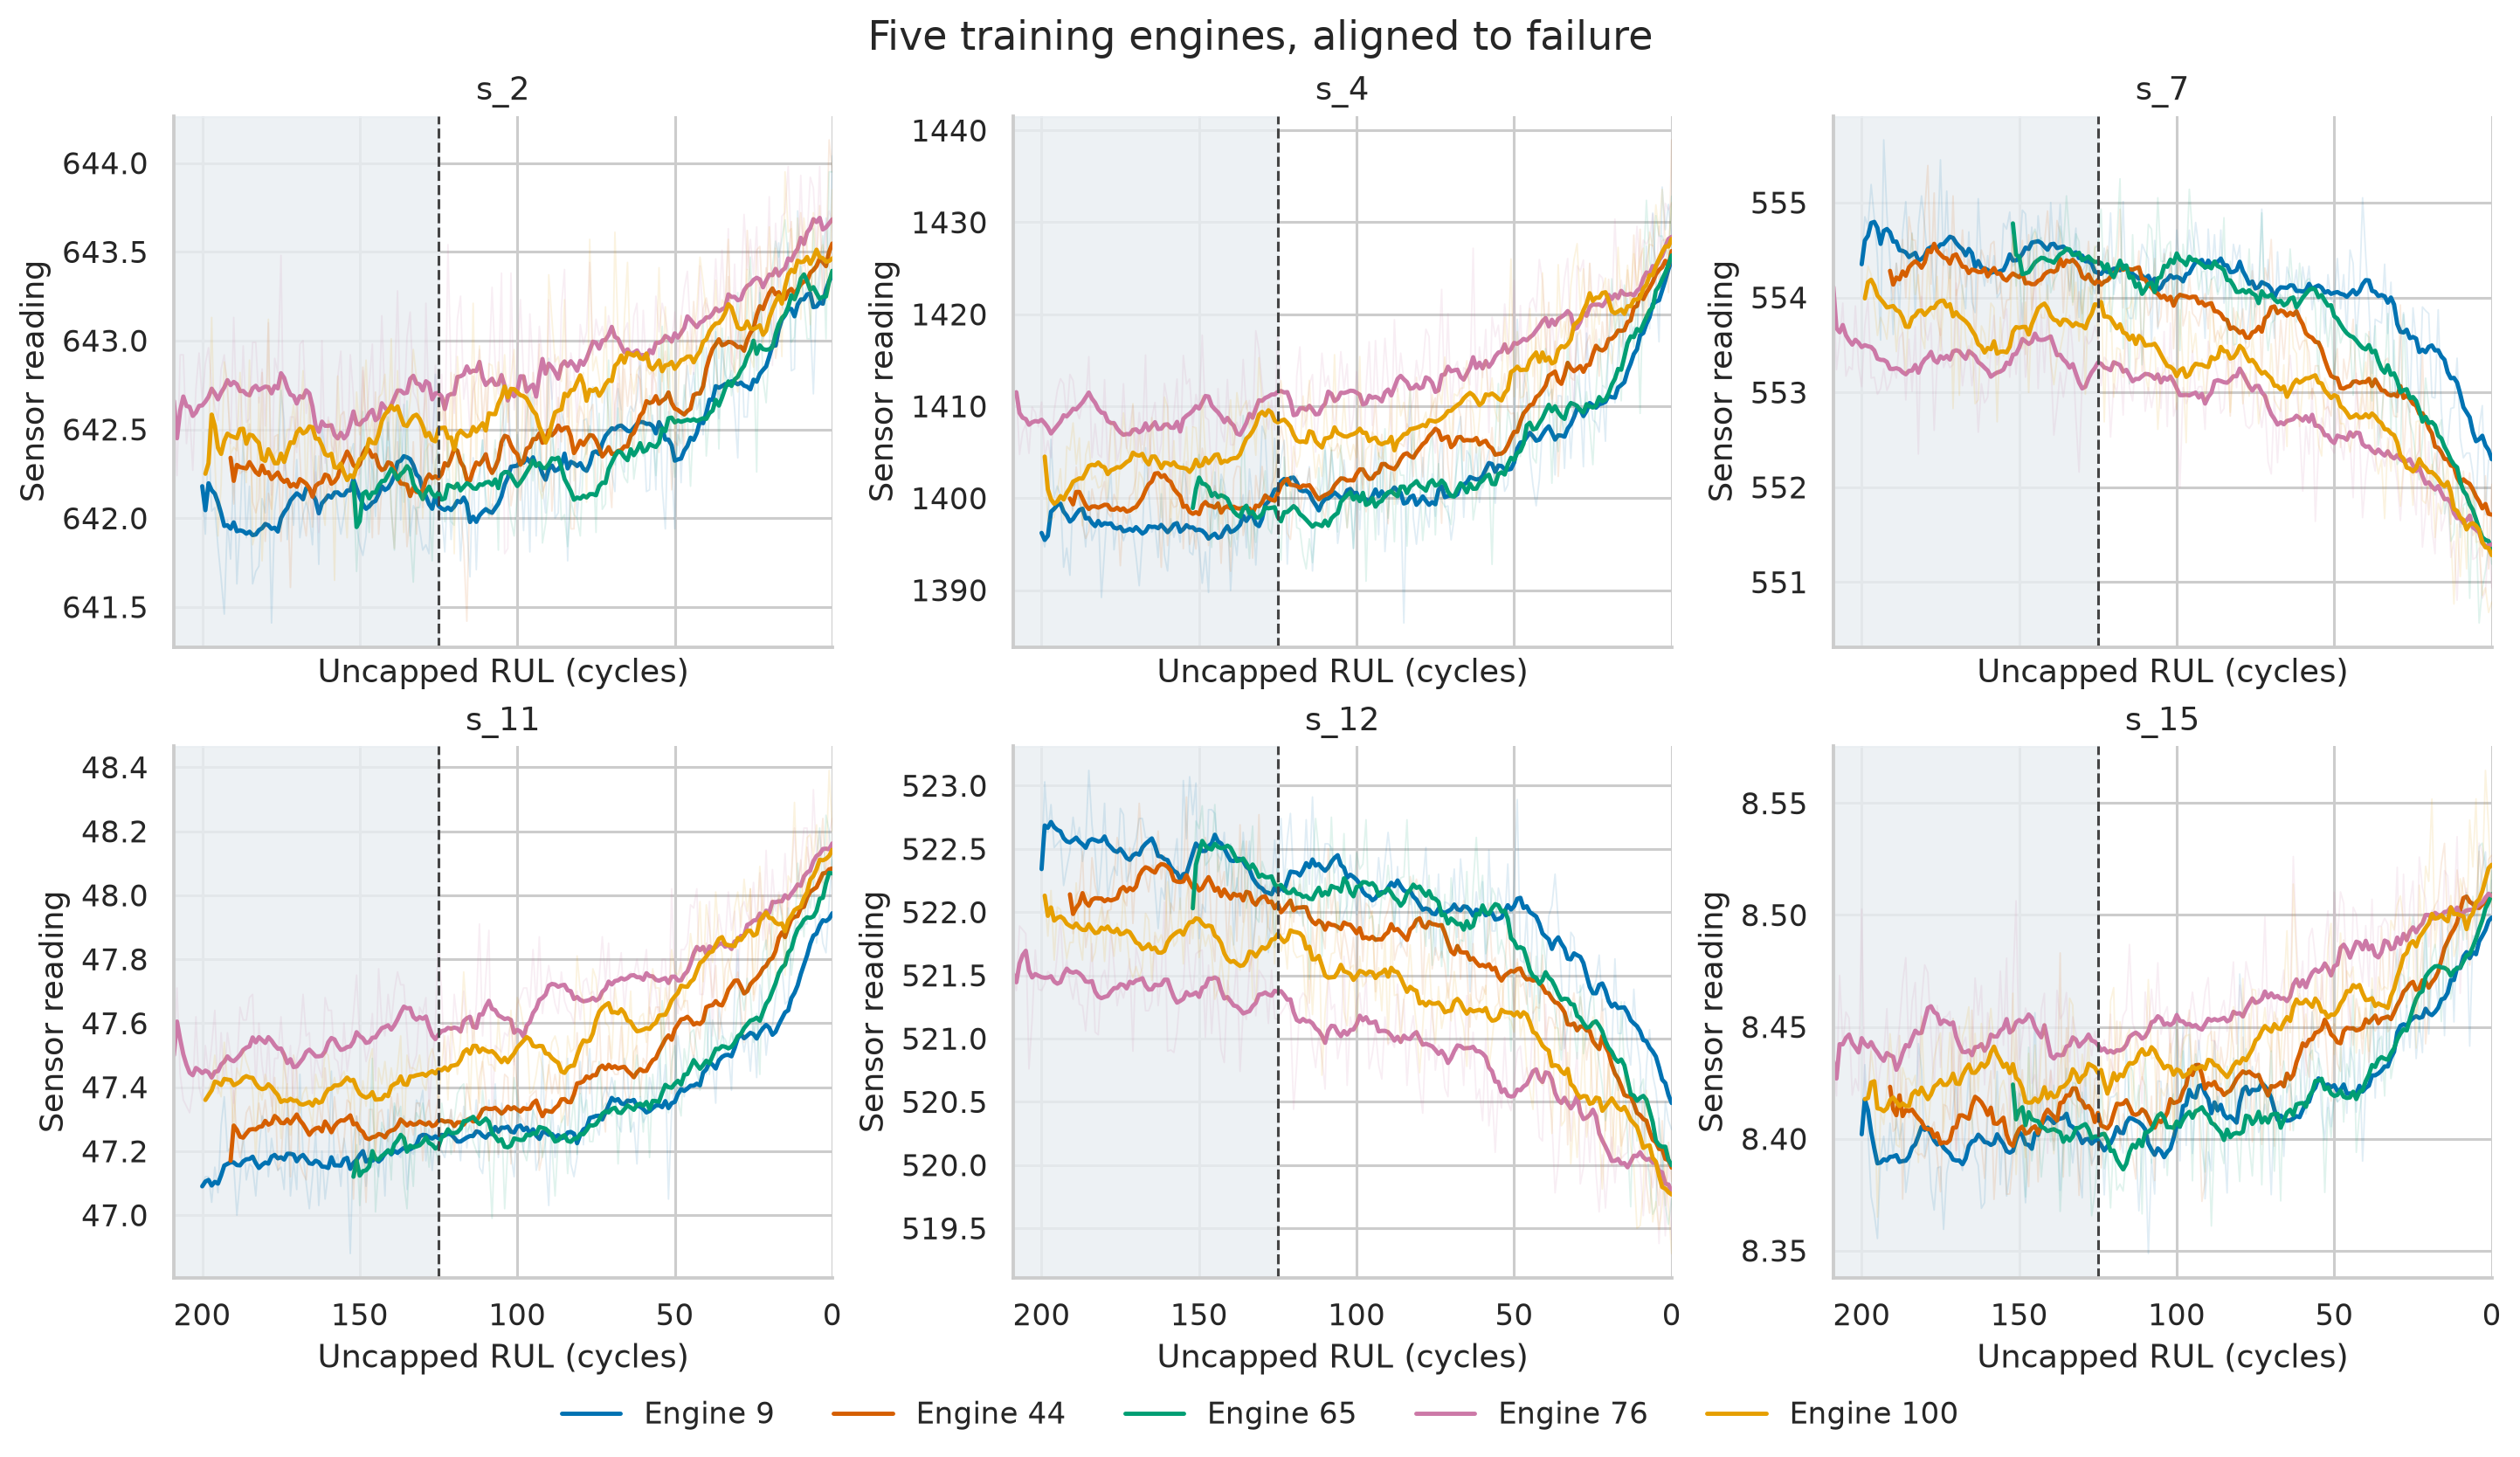
\includegraphics[width=\textwidth]{../figures/eda_sensor_trends.png}
  \caption{Six representative retained sensors from five training engines,
  aligned on uncapped RUL. Failure is at the right. The shaded area has
  RUL above 125; the dashed line marks the team's target cap.}
  \label{fig:eda-trends}
\end{figure*}

We adopt the training target $y_{i,t}=\min(125,r_{i,t})$. Liu, Wang and
Yu~\cite{liu2021rul}, Section 4.2, use an upper target limit of 125 on C-MAPSS
because early sensor evolution carries weak degradation information.
Our plots support this motivation but do not prove that early RUL is
unlearnable or that 125 is optimal. The cap changes 8,031 training labels
(38.93\%). A cap of 100 creates a longer plateau and removes more early-life
target resolution; no cap preserves exact targets but requires distinguishing
more early-life states. The modeling stage compares capped and uncapped
targets with engine-grouped cross-validation. True test RUL remains uncapped.

\subsection{Correlation and limitations}
Figure~\ref{fig:eda-correlation} reports Pearson correlations of the 14
retained sensors and both uncapped and 125-capped training RUL. Several sensors share substantial
variation. We do not remove a sensor solely for correlating with another;
its model-specific contribution requires subsequent evaluation. These are
pooled, row-weighted descriptive associations: adjacent cycles are dependent
and between-engine differences contribute. They do not demonstrate causation
or independent-sample significance, and weak linear association does not
exclude nonlinear or temporal information.

\begin{figure*}[t]
  \centering
  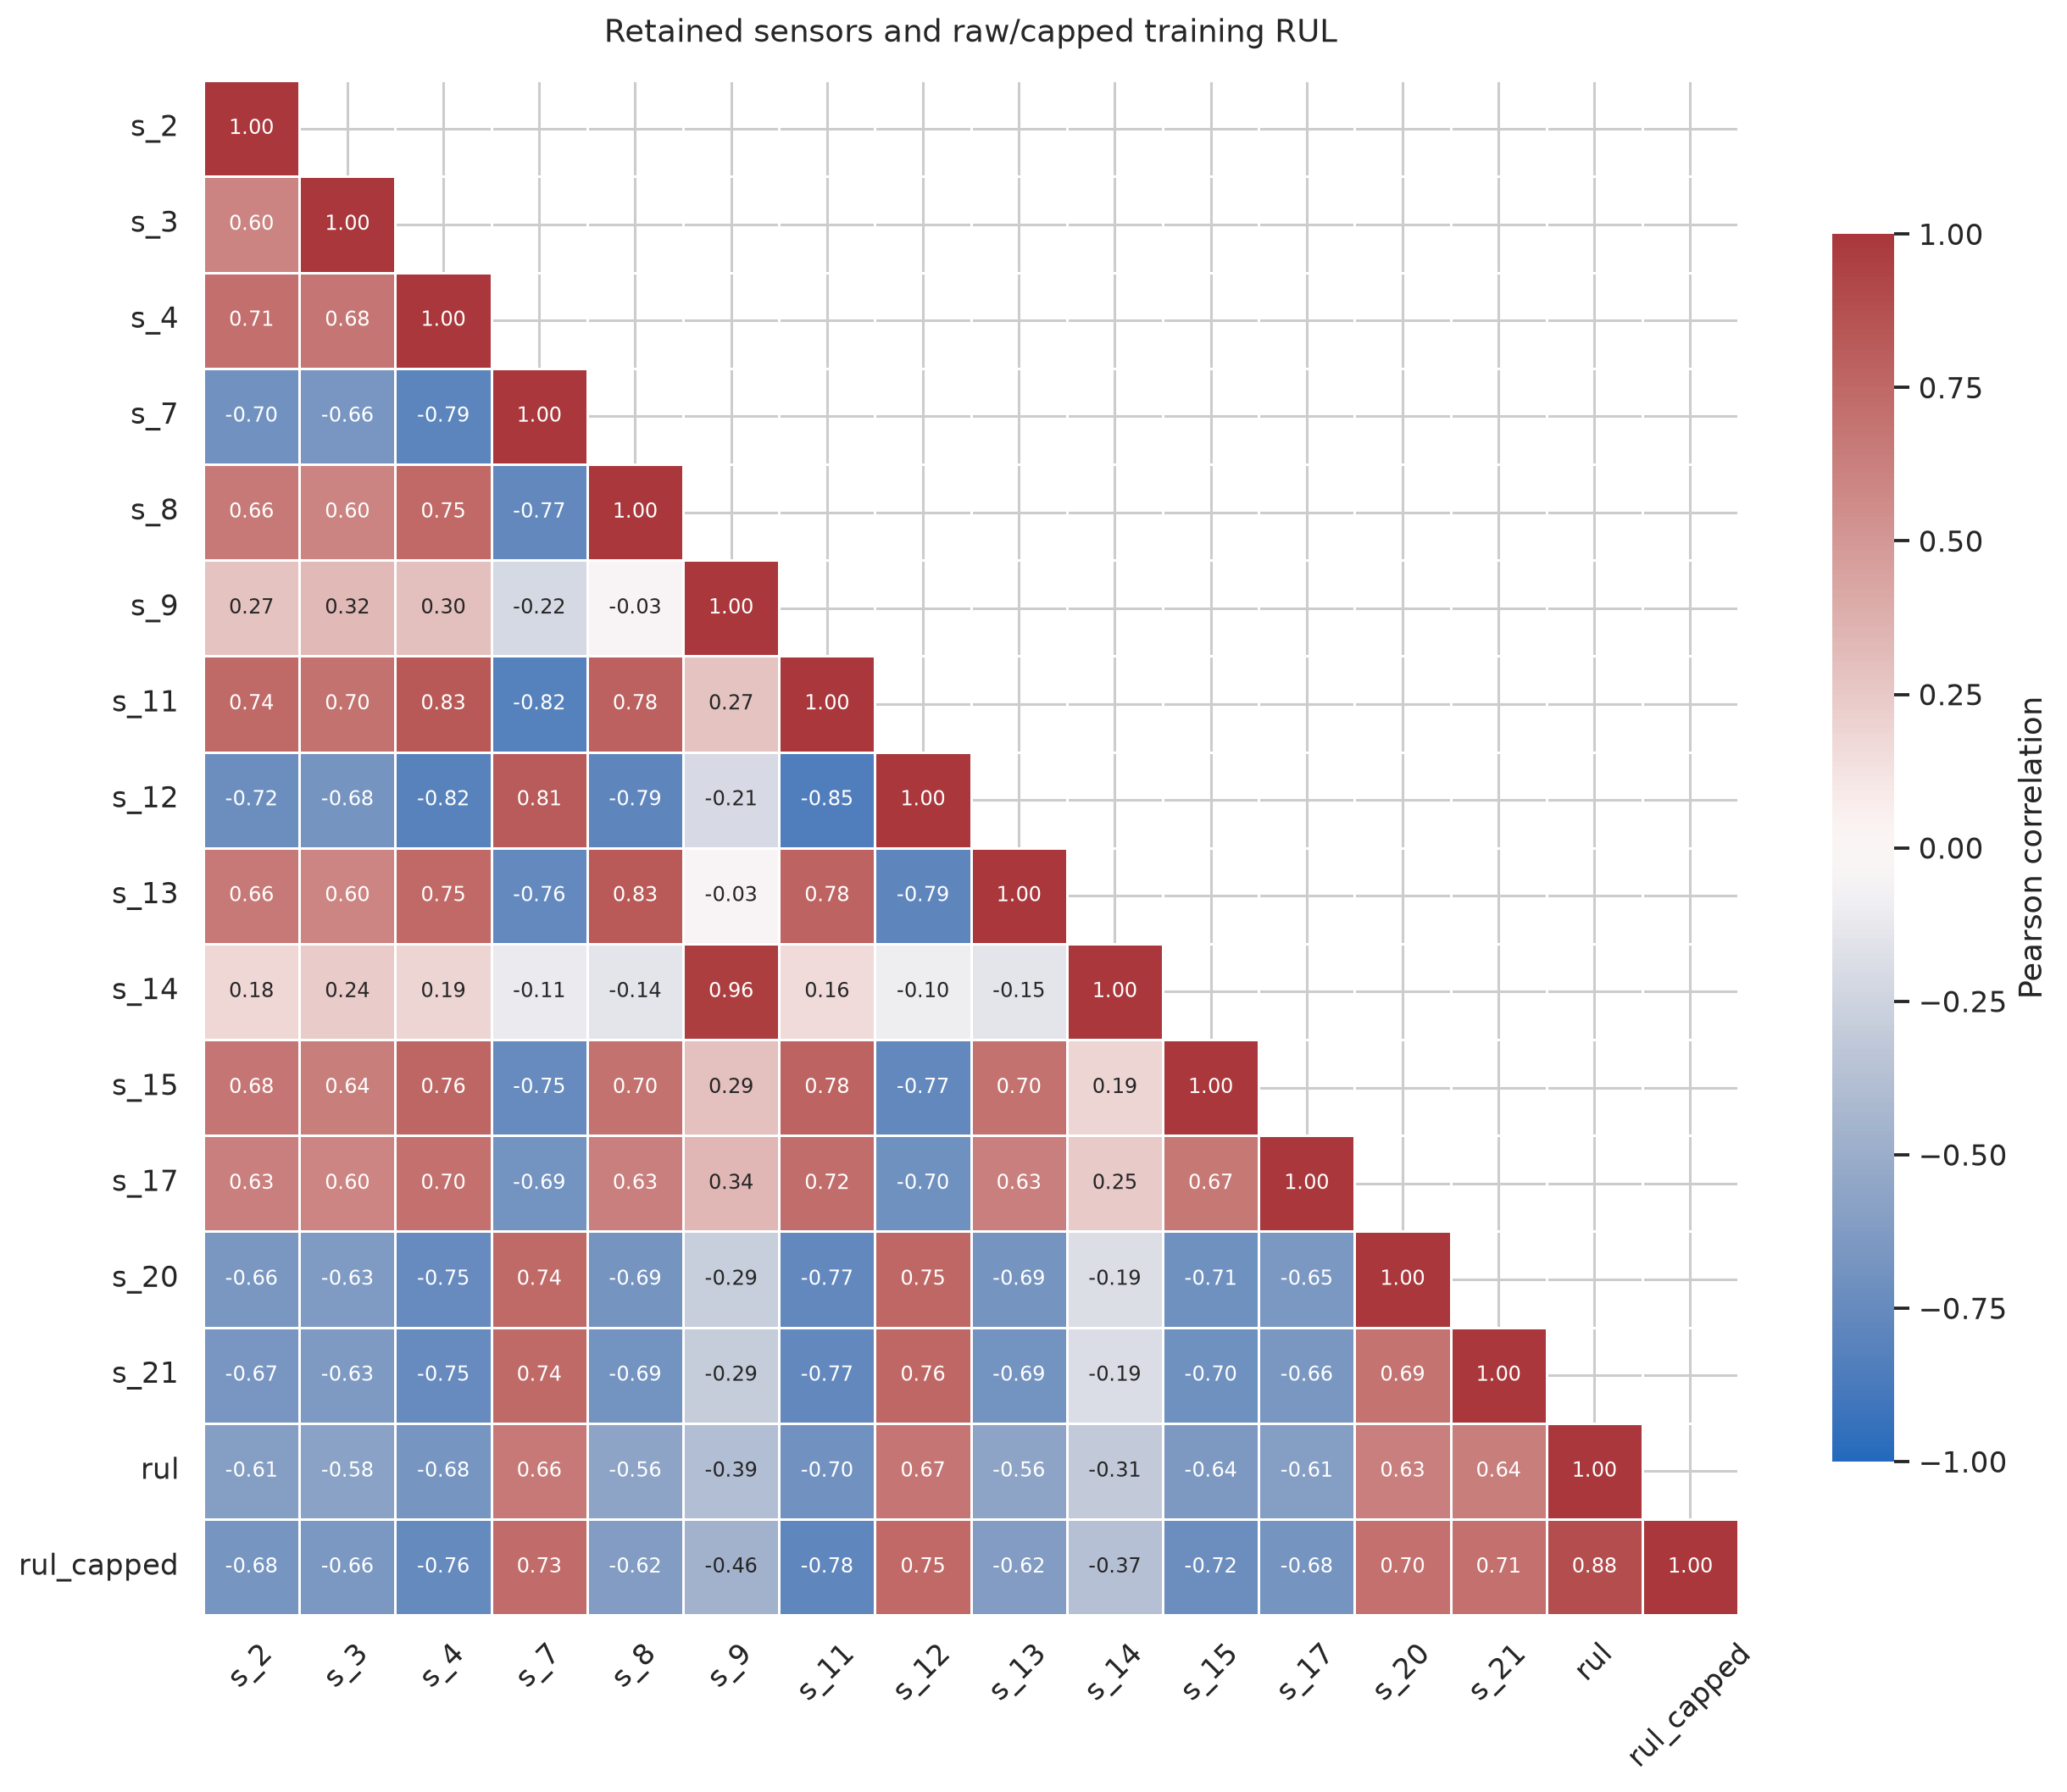
\includegraphics[width=0.85\textwidth]{../figures/eda_correlations.png}
  \caption{Pearson correlations of retained sensors with each other and
  uncapped and 125-capped training RUL. Constants are excluded because their correlations
  are undefined.}
  \label{fig:eda-correlation}
\end{figure*}

This analysis is specific to FD001 and simulated run-to-failure histories.
Sensor selection should be revisited for other operating conditions.
Any learned scaler or feature transformation used in cross-validation must
be fit within its training fold. The notebook retains its outputs and exports
the evidence tables to \texttt{results/eda\_*.csv} for reproducibility.


\subsection{Final descriptive test diagnostics}
After all preceding training decisions, we plot each test engine's last observed
cycle and the distribution of its supplied true RUL (Fig.~\ref{fig:eda-test}).
These are descriptive only; no earlier choice was revisited. Last observed cycle
is a truncation point, not failure or physical engine age. Labels remain uncapped.
No tuning, sensor selection or model evaluation uses these plots.

\begin{figure*}[t]
  \centering
  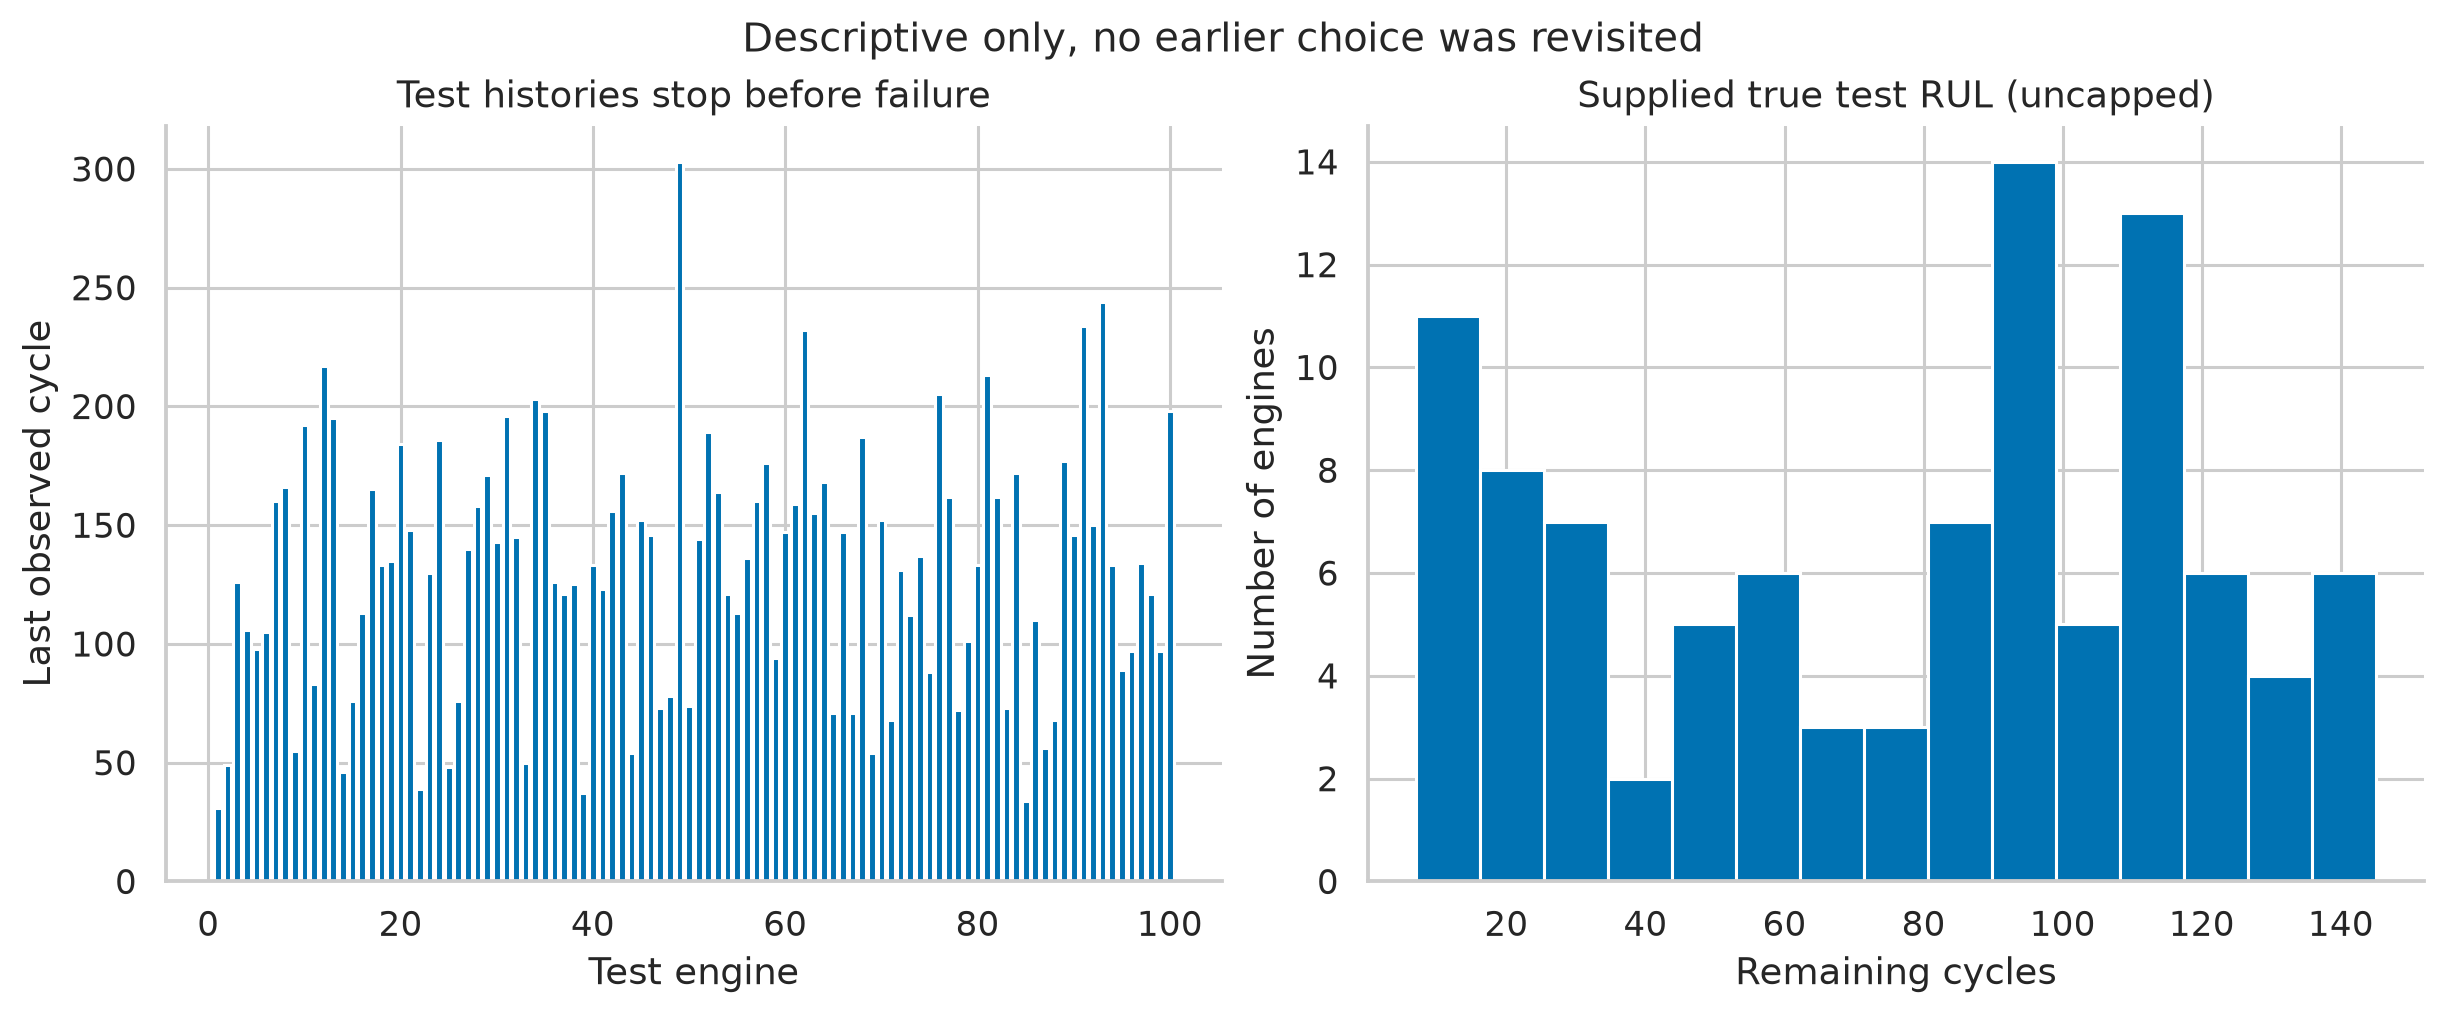
\includegraphics[width=\textwidth]{../figures/eda_test_diagnostics.png}
  \caption{Final test diagnostics: last observed cycle per engine and true RUL
  distribution. Descriptive only, no earlier choice was revisited.}
  \label{fig:eda-test}
\end{figure*}

% ABOUTME: Evaluation protocol section of the IEEE report (issue #2).
% ABOUTME: Engine level splitting, leakage, metric definitions and the early vs late stage split.
\section{Evaluation Protocol}
\label{sec:evaluation}

\subsection{Splitting by engine}
Each training engine in FD001 contributes one row per operating cycle, and
consecutive cycles of the same engine differ only by a small amount of
degradation and sensor noise. If rows were split at random, cycle $t$ of an
engine could fall in the training set while cycle $t+1$ fell in the
validation set. The model would then be scored on near copies of rows it had
already seen, and the validation error would understate the error on a new
engine. We therefore split by engine: every row of a given \texttt{unit} lies
on one side of the split only. Hyperparameters are tuned with five fold
\texttt{GroupKFold} cross validation grouped on \texttt{unit}, with a fixed
seed of 42. The test set is used once, after all hyperparameters are frozen.

\subsection{Scoring on test engines}
Training engines run to failure, but each test engine is cut off at an
unknown point before failure, and the dataset gives the true RUL only at its
last observed cycle. Each test engine is therefore scored once, using the
prediction at its final cycle, so all 100 test engines carry equal weight.

\subsection{Metrics}
Let $y_i$ be the true RUL of engine $i$, $\hat{y}_i$ the prediction,
$d_i = \hat{y}_i - y_i$ the error and $n$ the number of engines. We report
\begin{align}
\mathrm{RMSE} &= \sqrt{\tfrac{1}{n}\textstyle\sum_{i} d_i^2}, \qquad
\mathrm{MAE} = \tfrac{1}{n}\textstyle\sum_{i} \lvert d_i \rvert, \\
S &= \sum_{i} s_i, \quad
s_i =
\begin{cases}
e^{-d_i/13} - 1, & d_i < 0,\\
e^{d_i/10} - 1, & d_i \ge 0,
\end{cases}
\end{align}
where $S$ is the asymmetric scoring function of the PHM08 challenge
\cite{saxena2008damage}. RMSE penalises large errors more than MAE does,
and both treat early and late predictions alike. The score $S$ does not: a
prediction that overestimates RUL by 10 cycles costs as much as one that
underestimates it by 13, and the penalty grows exponentially. Overestimating
RUL means the engine is believed healthy when it is close to failure, which
risks an in service failure; underestimating it only brings maintenance
forward. Because $S$ is a sum rather than a mean, it is compared only across
models scored on the same set of engines.

\subsection{Early and late stage error}
Maintenance decisions are made near the end of an engine's life, so error
there matters more than error far from failure. We split the test engines by
true RUL into a late stage ($y_i \le 50$ cycles) and an early stage
($y_i > 50$) and report RMSE and MAE for each. A model with a good overall
RMSE but a poor late stage RMSE would be of little use for scheduling
maintenance.

% ABOUTME: Feature engineering section of the IEEE report (issue #4).
% ABOUTME: Rolling statistics, least squares slope, regime normalisation, health index, ablation.
\section{Degradation Features}
\label{sec:features}

Each FD001 row is one cycle of one engine: the cycle number, three
operating settings and 21 sensor readings. A single reading is noisy and
says little about how far an engine has degraded, so we add features that
summarise each sensor's recent history. All features are computed by
\texttt{make\_features} in \texttt{src/rul/features.py}, which returns one
row per input row with the original index. Every window is computed within
a single engine (grouped by \texttt{unit} and ordered by cycle), so no
feature ever mixes readings from two engines.

\subsection{Cycle}
The cycle number $t$ is kept unchanged as a feature. It is the time since
the engine entered service in the dataset, so on its own it is a weak prior
on wear. It is not scaled, since tree models are invariant to monotone
rescaling and downstream code uses the raw cycle.

\subsection{Operating regime normalisation}
Sensor levels depend on the flight condition (altitude, Mach number and
throttle angle) as much as on wear. We standardise the three settings and
cluster them with $k$-means (seed 42) into $K$ operating regimes. For each
regime $r$ and sensor $j$ we store the mean $\mu_{rj}$ and standard
deviation $\sigma_{rj}$ over the training rows in that regime, and
normalise
\begin{equation}
z_{t,j} = \frac{x_{t,j} - \mu_{r(t),j}}{\sigma_{r(t),j}},
\end{equation}
where $r(t)$ is the regime nearest to the row's settings. FD001 runs in one
regime ($K = 1$), so this is an ordinary z-score; with $K = 6$ the same code
removes the regime offsets of FD002 and FD004, leaving variation due to
wear. Sensors that are constant in FD001 (s\_1, s\_5, s\_10, s\_16, s\_18,
s\_19) have $\sigma = 0$ up to floating point noise; they are only centred,
so their features are zero rather than amplified noise.

The cluster centres and $(\mu, \sigma)$ are estimated on training engines
only and stored in a scaler object that is reused, unchanged, on
validation and test engines. If they were re-estimated on the validation
engines, the validation features would be scaled by statistics that
include those engines' own failure trajectories, and the cross validated
error would be optimistic. In cross validation the scaler is refitted in
every fold on that fold's training engines.

\subsection{Rolling mean and standard deviation}
For window length $w \in \{5, 10, 20\}$ and the set $W_t$ of the last
$\min(w, t)$ cycles of the same engine, with $n = |W_t|$,
\begin{equation}
m^{(w)}_{t,j} = \frac{1}{n}\sum_{s \in W_t} z_{s,j}, \qquad
s^{(w)}_{t,j} = \sqrt{\frac{1}{n - 1}\sum_{s \in W_t}
\bigl(z_{s,j} - m^{(w)}_{t,j}\bigr)^2}.
\end{equation}
The mean filters measurement noise and estimates the current level of
degradation; the standard deviation measures how erratic the sensor has
become, which tends to grow as components wear.

\paragraph{Early cycles} The first $w - 1$ cycles of an engine have fewer
than $w$ past readings. Rather than drop these rows or leave missing values,
the window is truncated to the cycles seen so far (\texttt{min\_periods=1}).
At cycle 1 the mean equals the reading and the standard deviation, undefined
for one value, is set to 0. These features are therefore noisier for the
first $w - 1$ cycles of each engine. Those cycles are at least 109 cycles
from failure in FD001, where the target is at or near the cap of 125, so
this costs little accuracy.

\subsection{Rolling least squares slope}
The slope is the ordinary least squares gradient of $z_{s,j}$ against cycle
$s$ over the same window. With $n$ points and sums taken over $W_t$,
\begin{equation}
b^{(w)}_{t,j} =
\frac{n \sum s\, z_{s,j} - \sum s \sum z_{s,j}}
     {n \sum s^2 - \bigl(\sum s\bigr)^2}.
\end{equation}
All five sums are rolling sums, so every slope is computed in closed form
in one pass instead of fitting a regression per row. For $n = 1$ the
denominator is zero and we define $b = 0$: a single point has no trend.

The slope is the local rate of degradation, in standard deviations per
cycle. The rolling mean says how worn an engine is; the slope says how fast
it is wearing. In FD001 the sensors drift slowly for most of an engine's
life and then accelerate as the fault develops, so a steep slope marks an
engine in the final phase of its life even when its sensor levels overlap
with those of a healthy engine of a different build. Because the slope uses
differences within one engine, it is also insensitive to the engine to
engine offsets in initial wear that make raw levels hard to compare. On a
window of 2 or 3 points the slope is dominated by noise, which is the main
cost of the truncated early windows.

\subsection{Health index}
The health index (HI) combines all normalised sensors into one number
between 0 and 1. We fit a linear regression on training engines,
\begin{equation}
h_t = 1 - \frac{t - 1}{T - 1}, \qquad
\widehat{\mathrm{HI}}_t = \mathrm{clip}\bigl(\beta_0 + \boldsymbol\beta^\top
\mathbf{z}_t,\ 0,\ 1\bigr),
\end{equation}
where $T$ is the engine's failure cycle, so the target $h$ falls linearly
from 1 at the first cycle to 0 at failure. At prediction time no $T$ is
needed: the fitted coefficients map any engine's sensors to an HI. We chose
regression over the first principal component because PCA finds the
direction of greatest variance, which need not be the direction of wear,
and its sign and scale are arbitrary; the regression picks the sensor
combination that tracks degradation directly and has a fixed 0 to 1 scale.
Its limitation is the linear target: real wear is flat for most of a life
and then accelerates, so the HI starts near 0.8 rather than 1 and only
falls clearly in the last third of life. On FD001 the HI has a correlation
of 0.86 with the capped RUL, higher than any single sensor (at most 0.80 in
absolute value for a 20 cycle rolling mean).

\subsection{Ablation}
Table~\ref{tab:feature-ablation} adds the feature families one at a time
to a Random Forest (default hyperparameters, seed 42), scored with five
fold cross validation grouped by engine on every validation cycle.

\begin{table}[t]
\centering
\caption{Feature ablation, 5 fold engine cross validation on FD001 training
engines (mean over folds, RUL capped at 125).}
\label{tab:feature-ablation}
\begin{tabular}{lrrrr}
\hline
Features & $n$ & RMSE & MAE & Late RMSE \\
\hline
Cycle and raw sensors      &  22 & 16.81 & 11.53 & 15.56 \\
+ rolling mean and std     & 148 & 16.35 & 11.02 & 13.87 \\
+ rolling slope            & 211 & 14.78 & 10.02 & 11.35 \\
+ health index             & 212 & 14.72 &  9.94 & 11.22 \\
\hline
\end{tabular}
\end{table}

Smoothing helps a little: a forest already averages over many noisy rows.
The slope gives the largest gain, about 1.6 RMSE and 2.5 late stage RMSE,
well beyond the fold to fold standard deviation of 0.5 to 0.8. The HI adds
a further small gain within that noise, since it is a linear combination of
sensors the forest already sees; its main value is as one interpretable
degradation signal.

\subsection{Limitation of fixed windows}
Every feature here looks back at most 20 cycles, while FD001 engines run
for 128 to 362 cycles. A fixed window cannot tell whether a sensor has been
drifting for 150 cycles or has just started to move, cannot see when the
drift began to accelerate, and must use one window length for engines that
degrade at very different rates. Lengthening the window trades this
against slower response and longer truncated starts, and the choice of
windows (5, 10, 20) is itself a hand-tuned hyperparameter. These are the
gaps that motivate Phase 2: sequence models such as LSTMs or temporal
convolutions take the whole trajectory as input and learn which part of
the history matters, rather than relying on fixed hand-made summaries.

% ABOUTME: Models and tuning section of the IEEE report (issue #5).
% ABOUTME: Elastic Net, Random Forest and XGBoost theory, tuning setup, CV results and the RUL cap.
\section{Models and Tuning}
\label{sec:models}

Each training row is one cycle of one engine, and the task is to regress
its RUL, capped at 125 cycles. We compare two naive baselines with three
models of increasing flexibility: Elastic Net, a regularised linear model;
Random Forest, an average of deep trees; and XGBoost, a sum of shallow
boosted trees. Each model is trained on two feature sets: the raw set
(cycle number and the 14 informative sensors, 15 features) and the
engineered set of Section~\ref{sec:features} (142 features). All models are
built by \texttt{build\_model} in \texttt{src/rul/models.py}. Random
Forest and XGBoost are seeded with 42; Elastic Net has no random component,
since its coordinate descent updates the coefficients in a fixed cyclic
order.

\subsection{Baselines}
The mean predictor returns the mean training RUL for every row; it ignores
the sensors and sets the error that any useful model must improve on.
Ordinary least squares on the raw features is the simplest model that uses
the sensors. Every tuned model is expected to beat both. Linear regression
is also fitted on the engineered features, as an unregularised reference
for Elastic Net on the same inputs.

\subsection{Elastic Net}
Elastic Net~\cite{zou2005elasticnet} is linear regression with a penalty
that mixes the L1 and L2 norms of the coefficients. In the parametrisation
used by scikit-learn, with $n$ rows, features $\mathbf{x}_i$ and targets
$y_i$, it solves
\begin{equation}
\begin{aligned}
\min_{\beta_0, \boldsymbol\beta}\ &
\frac{1}{2n}\sum_{i=1}^{n}\bigl(y_i - \beta_0 - \boldsymbol\beta^\top
\mathbf{x}_i\bigr)^2 \\
& + \alpha\rho\,\lVert\boldsymbol\beta\rVert_1
+ \frac{\alpha(1-\rho)}{2}\,\lVert\boldsymbol\beta\rVert_2^2 ,
\end{aligned}
\end{equation}
where $\alpha \ge 0$ sets the overall strength of the penalty and
$\rho \in [0, 1]$ (\texttt{l1\_ratio}) its L1 share. The L1 term can set
coefficients exactly to zero, so it selects features. On its own (the
Lasso, $\rho = 1$) it tends to keep one feature from a group of correlated
features and drop the others more or less arbitrarily, and the choice can
change between samples. The L2 term shrinks coefficients smoothly towards
zero, spreads weight across correlated features and makes the solution
stable. Mixing the two gives sparse models that remain stable when
features are strongly correlated, as the rolling statistics of one sensor
over three windows are.

The penalty depends on the scale of each coefficient, so features are
standardised first. The scaler and the regression form one scikit-learn
\texttt{Pipeline}, so in cross validation the scaler is fitted on each
fold's training engines only. Elastic Net is linear in its inputs, so it
has high bias and low variance. On raw sensors it cannot follow the
flat-then-accelerating shape of degradation; it can represent nonlinear
behaviour only through features that already encode it, such as rolling
slopes and the health index. The penalty lowers variance further at the
cost of more bias.

\subsection{Random Forest}
A regression tree splits the feature space into boxes and predicts the mean
target in each box. A deep tree has low bias but high variance: a small
change in the training data can change its splits completely. Random
Forest~\cite{breiman2001rf} trains $B$ trees, each on a bootstrap sample of
the rows (bagging), considers only a random subset of the features at each
split, and averages the predictions. If each tree has variance $\sigma^2$
and two trees have correlation $\rho$, the variance of the average is
\begin{equation}
\rho\,\sigma^2 + \frac{1-\rho}{B}\,\sigma^2 .
\end{equation}
Adding trees removes the second term, and sampling features at each split
lowers $\rho$, so the forest keeps the low bias of deep trees while
reducing their variance. Trees are trained independently, and as trees
are added the forest's generalisation error converges~\cite{breiman2001rf}:
adding trees does not increase overfitting; the error levels off, so more
trees only cost time.

\subsection{Gradient boosting and XGBoost}
Boosting builds an additive model one tree at a time, each tree correcting
the errors of the trees before it~\cite{friedman2001gbm}:
\begin{equation}
F_m(\mathbf{x}) = F_{m-1}(\mathbf{x}) + \eta\, f_m(\mathbf{x}),
\end{equation}
where $f_m$ is a shallow tree fitted to the negative gradient of the loss
at $F_{m-1}$ and $\eta$ is the learning rate. For squared error the
negative gradient is the residual $y_i - F_{m-1}(\mathbf{x}_i)$, so each
tree is fitted to what the current model still gets wrong. Where bagging
averages independent low-bias trees to cut variance, boosting adds
dependent high-bias trees to cut bias. Each added tree fits the training
data more closely, so the number of rounds, the learning rate and the tree
depth must be limited to control variance.

XGBoost~\cite{chen2016xgboost} adds regularisation to the boosting
objective. Tree $m$ minimises
\begin{equation}
\sum_{i=1}^{n} \ell\bigl(y_i, F_{m-1}(\mathbf{x}_i) + f_m(\mathbf{x}_i)\bigr)
+ \gamma T + \frac{\lambda}{2}\lVert\mathbf{w}\rVert_2^2 ,
\end{equation}
where $T$ is the number of leaves and $\mathbf{w}$ the leaf values. The
$\gamma$ term charges for each extra leaf, and the $\lambda$ term
(\texttt{reg\_lambda}) shrinks leaf values, so a leaf supported by few rows
moves the prediction less. XGBoost uses a second order Taylor expansion of
the loss to choose splits and leaf values, and can also subsample rows
(\texttt{subsample}) and features (\texttt{colsample\_bytree}) for each
tree, which adds bagging-like randomness.

\subsection{Tuning setup}
All tuning uses the five engine-grouped folds of
Section~\ref{sec:evaluation}, so every engine is validated exactly once and
no engine appears on both sides of a split. The engineered features depend
on statistics fitted to training data; they are rebuilt in every fold from
that fold's training engines and then applied to its validation engines.
Each model is tuned separately on each feature set, and the configuration
with the lowest mean validation RMSE is selected. Elastic Net is cheap, so
its full grid is searched; for Random Forest and XGBoost a fixed number of
configurations is drawn at random from the grid with seed 42.
Table~\ref{tab:search-space} lists the search spaces and the selected
values. The test set is not used.

\begin{table}[t]
\centering
\caption{Search spaces. Selected values are in parentheses, given as
raw / engineered where the two feature sets differ. Random Forest and
XGBoost sample 6 and 8 configurations from their grids; Elastic Net
searches all 12.}
\label{tab:search-space}
\footnotesize
\begin{tabular}{llp{2.9cm}}
\hline
Model & Hyperparameter & Values (selected) \\
\hline
Elastic Net & \texttt{alpha} & 0.1, 0.3, 1.0 (0.1) \\
            & \texttt{l1\_ratio} & 0.2, 0.5, 0.8, 1.0 (1.0) \\
\hline
Random      & \texttt{n\_estimators} & 100, 200 (200 / 100) \\
Forest      & \texttt{max\_depth} & 8, 12, none (12 / none) \\
            & \texttt{min\_samples\_leaf} & 1, 5, 10 (1 / 5) \\
            & \texttt{max\_features} & 0.3, 0.5, 1.0 (0.3 / 0.5) \\
\hline
XGBoost     & \texttt{n\_estimators} & 200, 400 (400) \\
            & \texttt{learning\_rate} & 0.03, 0.05, 0.1 (0.03 / 0.05) \\
            & \texttt{max\_depth} & 3, 4, 6 (4) \\
            & \texttt{subsample} & 0.8, 1.0 (1.0) \\
            & \texttt{colsample\_bytree} & 0.5, 0.8, 1.0 (0.5 / 0.8) \\
            & \texttt{reg\_lambda} & 1, 5 (5) \\
\hline
\end{tabular}
\end{table}

\subsection{Cross validation results}
Table~\ref{tab:cv-results} reports each selected configuration. RMSE and
MAE are the mean and standard deviation over the five folds, computed on
every held-out cycle against the capped target. Late RMSE restricts the
error to cycles with true RUL of at most 50, and the last column to cycles
with true RUL of at most 125, where capped and true labels agree.

These are model-selection scores. The same folds are used to choose each
configuration and to report its score, so the scores of the selected
configurations are optimistic: among several configurations, the one that
did best on these folds is partly the one that was luckiest on them.
Grouping by engine prevents leakage between engines, and a small search
averaged over five folds limits the optimism, but neither removes this
selection bias. Nested cross validation would remove it; here the
independent estimate comes instead from the test set, which is scored once
with the frozen configurations (Section~\ref{sec:evaluation}).

\begin{table*}[t]
\centering
\caption{Five fold engine cross validation on FD001 training engines. Rows
above the line are trained on RUL capped at 125 and scored against it. The
two rows below the line retrain the best configuration with and without the
cap and score both against the true RUL, so their RMSE and MAE are
comparable with each other but not with the rows above; the last column is
comparable across all rows.}
\label{tab:cv-results}
\small
\begin{tabular}{lllrrrr}
\hline
Model & Features & Target & RMSE & MAE & Late RMSE & RMSE, RUL $\le 125$ \\
\hline
Mean baseline     & --         & capped   & $41.67 \pm 0.00$ & $36.97 \pm 0.00$ & 63.56 & 43.76 \\
Linear regression & raw        & capped   & $20.12 \pm 1.54$ & $16.37 \pm 1.29$ & 21.71 & 20.79 \\
Elastic Net       & raw        & capped   & $20.12 \pm 1.54$ & $16.37 \pm 1.29$ & 21.72 & 20.78 \\
Random Forest     & raw        & capped   & $16.43 \pm 0.77$ & $11.47 \pm 0.71$ & 15.40 & 18.29 \\
XGBoost           & raw        & capped   & $16.42 \pm 0.87$ & $11.38 \pm 0.70$ & 15.23 & 18.28 \\
Linear regression & engineered & capped   & $17.07 \pm 0.78$ & $13.72 \pm 0.63$ & 16.89 & 17.65 \\
Elastic Net       & engineered & capped   & $17.75 \pm 1.06$ & $14.33 \pm 0.85$ & 17.63 & 18.15 \\
Random Forest     & engineered & capped   & $14.42 \pm 0.48$ & $9.87 \pm 0.56$  & 10.98 & 15.76 \\
XGBoost           & engineered & capped   & $\mathbf{13.99} \pm 0.46$ & $\mathbf{9.81} \pm 0.42$ & \textbf{9.88} & \textbf{15.09} \\
\hline
XGBoost           & engineered & capped   & $47.47 \pm 2.21$ & $30.38 \pm 0.77$ & 9.88  & 15.09 \\
XGBoost           & engineered & uncapped & $38.26 \pm 1.41$ & $26.16 \pm 1.65$ & 11.20 & 25.99 \\
\hline
\end{tabular}
\end{table*}

Engineered features improve every model, by 2.0 to 2.4 RMSE, well beyond
the fold standard deviations. The tree ensembles beat the linear models by
a wide margin on both feature sets. Degradation in the sensors is
nonlinear and accelerates near failure. A linear model can follow this only
to the extent that its features already encode it: the rolling statistics,
slopes and health index supply part of that structure, which is why linear
regression improves from 20.12 to 17.07 with them. Trees learn the
remaining nonlinearity directly, piece by piece. XGBoost on
engineered features has the lowest error on every metric, though Random
Forest is within one fold standard deviation on overall RMSE; XGBoost's
clearer advantage is on late-life cycles (9.88 against 10.98).

All tuned models beat the mean baseline. Against the linear regression
baseline on raw features, both tree ensembles are better on both feature
sets and Elastic Net is better on engineered features (17.75 against
20.12). On raw features Elastic Net and linear regression are tied:
Elastic Net's RMSE is 0.0006 lower and its MAE 0.0015 higher, far inside
the fold standard deviation. With 15 features and over 16,000 training
rows per fold, the linear model is limited by bias rather than variance,
so the penalty has almost nothing to remove, and at small $\alpha$ Elastic
Net reduces to least squares. On engineered features, Elastic Net is less
accurate than unregularised linear regression on the same features (17.75
against 17.07). The selected penalty is pure L1, which makes the model
sparse by setting some coefficients exactly to zero, but it does not
improve predictive accuracy here; Elastic Net's gain over the raw baseline
comes from the engineered features, not from regularisation.

\subsection{Effect of the RUL cap}
Capping assumes that degradation is not visible early in life, so a model
should not be asked to tell 300 remaining cycles from 200. To test this,
the best configuration was retrained on the uncapped RUL with the same
folds, and both versions were scored against the true RUL (the last two
rows of Table~\ref{tab:cv-results}). The answer depends on which cycles
are scored. On cycles with true RUL of at most 125, the capped model is
far more accurate (RMSE 15.09 against 25.99), and it is also better on
late-life cycles (9.88 against 11.20). Over all cycles the uncapped model
is better (38.26 against 47.47). The capped model never sees a training
target above 125, so its predictions for young engines stay close to 125
while their true RUL is several hundred cycles. Capping changes the
training target rather than bounding the predictions: it concentrates the
model on the part of life where degradation is visible, trading accuracy
on early-life cycles, where predictions have little practical use, for
accuracy close to failure, where maintenance decisions are made. We keep
the cap for all models.

\subsection{Selected model}
XGBoost on engineered features, trained on RUL capped at 125, is carried
forward to the test set with the hyperparameters in
Table~\ref{tab:search-space}. The selected configuration of every model on
both feature sets is saved in \texttt{results/best\_params.json}, together
with the sensor list and window lengths needed to rebuild the features, so
test evaluation uses exactly the configurations chosen here.

% ABOUTME: Test set results section of the IEEE report (issue #6).
% ABOUTME: Frozen models scored once on FD001 test engines, error analysis and published comparison.
\section{Test Set Results}
\label{sec:results}

\subsection{Protocol}
Every hyperparameter and the choice of selected model were fixed by cross
validation (Section~\ref{sec:models}) before the test set was opened. Each
configuration is refitted on all 100 training engines with RUL capped at
125 cycles, and the feature statistics (regime normalisation and the health
index) are fitted on the training engines and applied unchanged to the test
engines. Features are computed over each test engine's full observed
history, and the model predicts once per engine at its last observed cycle
(Section~\ref{sec:evaluation}). Predictions are scored against the true,
uncapped RUL. All numbers in this section are taken from
\texttt{results/test\_metrics.csv}.

\begin{table*}[t]
\centering
\caption{Test results on the 100 FD001 test engines, scored against the
true RUL. Late stage is true RUL $\le 50$ (33 engines), early stage is
true RUL $> 50$ (67 engines). XGBoost on engineered features was selected
by cross validation before the test set was used.}
\label{tab:test-results}
\begin{tabular}{llrrrrrr}
\hline
Model & Features & RMSE & MAE & Score $S$ & Early RMSE & Late RMSE & Late MAE \\
\hline
Mean baseline     & --         & 43.07 & 35.90 & 33629 & 27.30 & 64.09 & 62.68 \\
Linear regression & raw        & 22.54 & 17.73 & 1291  & 21.93 & 23.72 & 19.83 \\
Elastic Net       & raw        & 22.57 & 17.77 & 1296  & 21.93 & 23.82 & 19.95 \\
Random Forest     & raw        & 17.77 & 13.21 & 534   & 19.42 & 13.83 & 8.90 \\
XGBoost           & raw        & 17.58 & 13.01 & 539   & 19.39 & 13.17 & 8.22 \\
Linear regression & engineered & 18.23 & 14.10 & 519   & 19.69 & 14.85 & 12.68 \\
Elastic Net       & engineered & 18.27 & 14.11 & 522   & 19.75 & 14.83 & 12.64 \\
Random Forest     & engineered & 15.23 & 11.33 & 344   & 17.88 & 7.34  & 5.06 \\
XGBoost (selected) & engineered & 15.36 & 11.26 & 389  & 18.11 & 7.03  & 5.25 \\
\hline
\end{tabular}
\end{table*}

\subsection{Overall results}
Table~\ref{tab:test-results} gives the results. The selected XGBoost model
reaches an RMSE of 15.36 cycles, an MAE of 11.26 and a score of 389. In the
late stage, where maintenance is scheduled, its RMSE is 7.03 cycles.
Random Forest is slightly better on the test set (RMSE 15.23, score 344),
although cross validation had ranked XGBoost first (13.99 against 14.42).
We keep the selection, because changing it after seeing test results would
make the test set a second validation set and bias the reported error
downwards.

With only 100 test engines, a gap this small may be sampling noise. A
paired bootstrap, resampling the 100 engines 10{,}000 times and scoring
both models on the same resample, gives a 95\% interval of $-1.3$ to
$+1.1$ cycles for the RMSE of Random Forest minus XGBoost, so the two
ensembles cannot be separated. The intervals for XGBoost minus Elastic Net
($-4.8$ to $-1.0$) and for XGBoost on engineered minus raw features
($-4.4$ to $-0.2$) exclude zero. The two conclusions of cross validation
therefore hold on unseen engines: tree ensembles beat the linear models,
and the engineered features improve every model, most of all in the late
stage, where XGBoost's RMSE falls from 13.17 to 7.03.

\begin{figure*}[t]
  \centering
  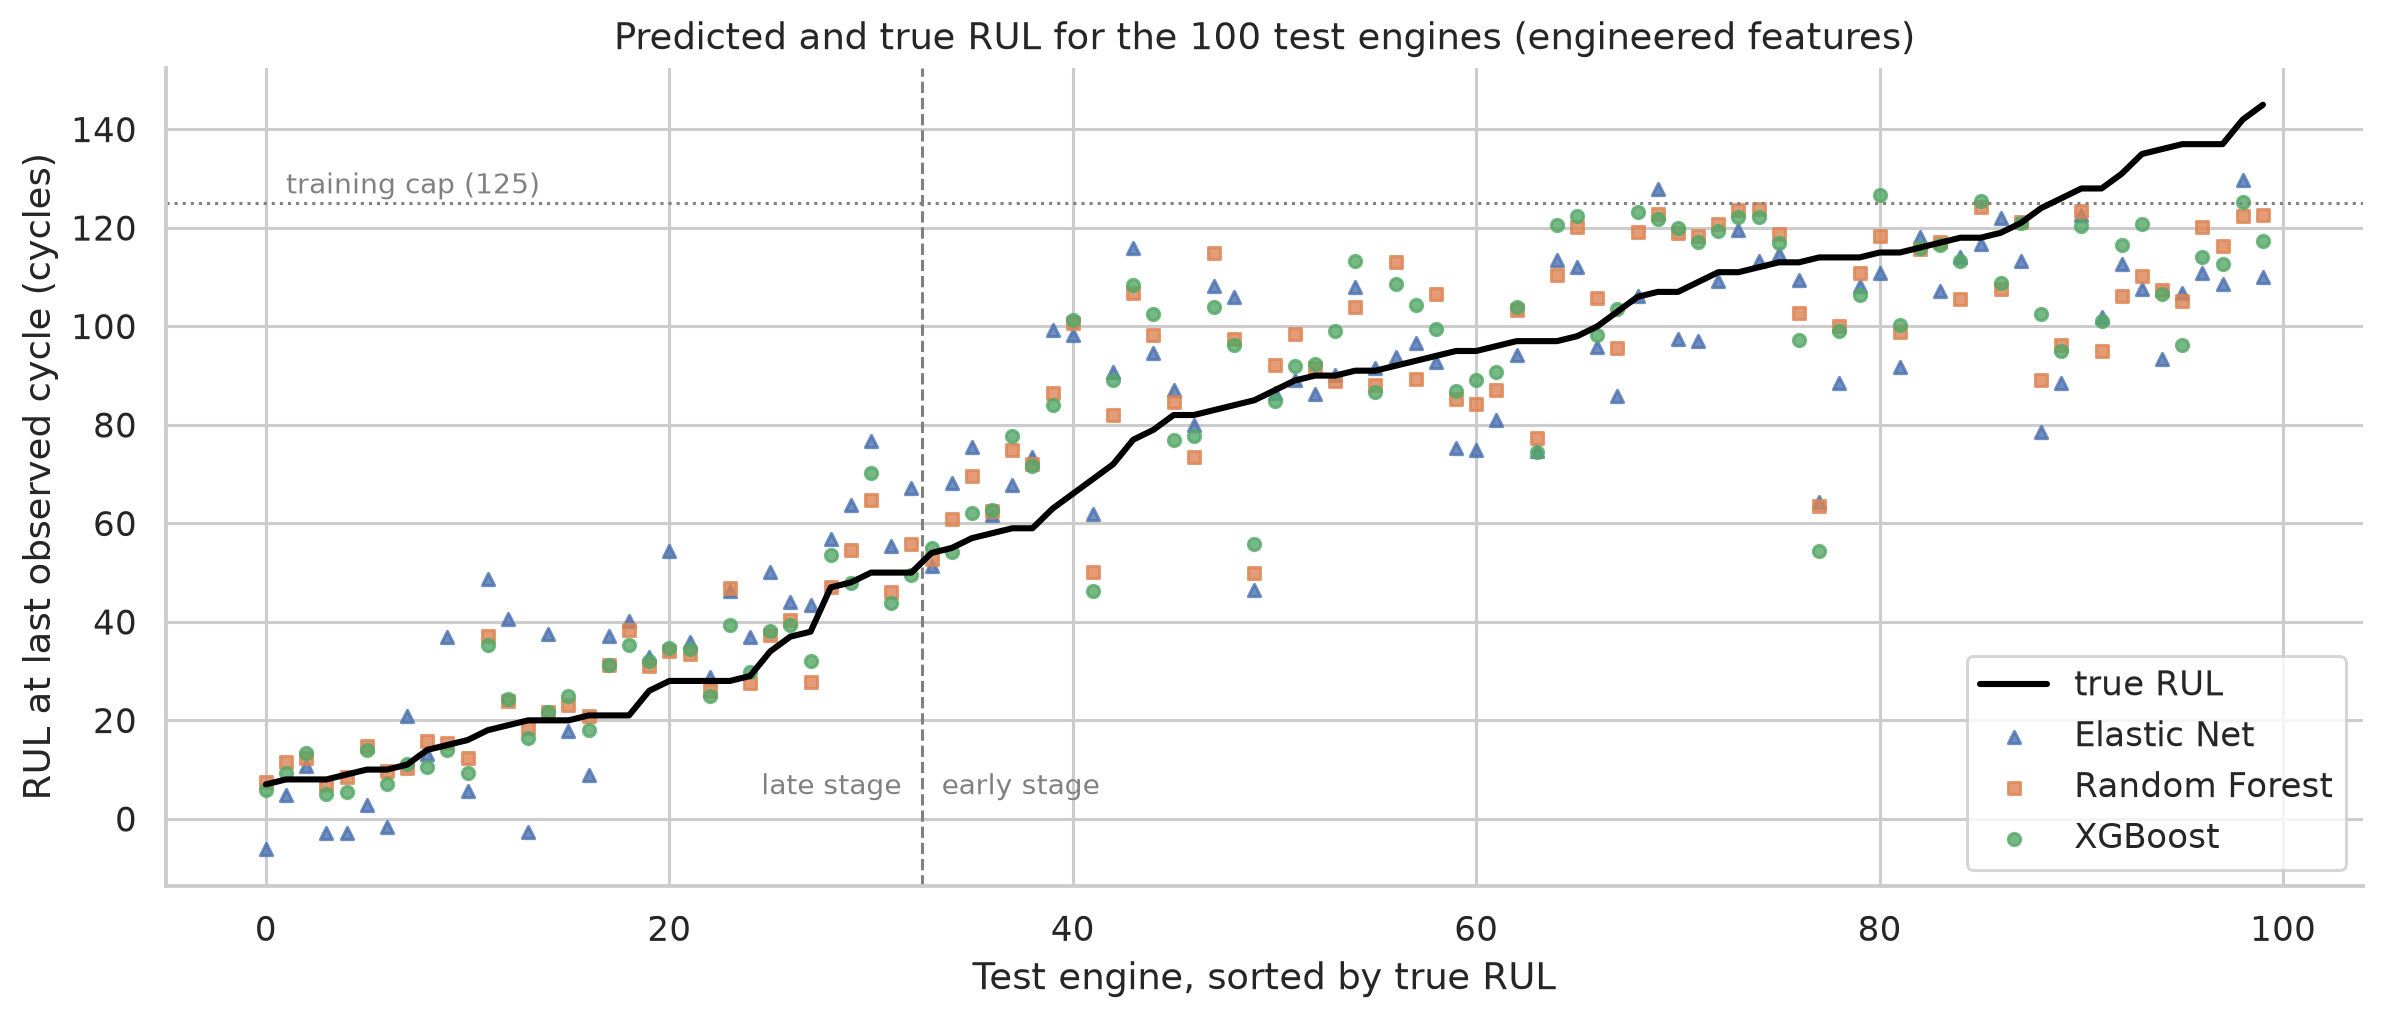
\includegraphics[width=\textwidth]{../figures/results_pred_vs_true.png}
  \caption{Predicted and true RUL at the last observed cycle of each test
  engine, sorted by true RUL. The dashed line separates the late stage
  (left) from the early stage; the dotted line is the training cap.}
  \label{fig:results-pred}
\end{figure*}

\subsection{Where the errors are}
Fig.~\ref{fig:results-pred} and Fig.~\ref{fig:results-buckets} show how
the error depends on the true RUL. For both tree ensembles the error is
smallest close to failure, with RMSE of about 7 cycles for true RUL of at
most 25 and about 8 between 26 and 50. It rises to between 16 and 17.5
cycles from 51 to 125. Elastic Net is close to the ensembles far from
failure but about twice as inaccurate in the late stage, which is where the
trees gain most. Between 51 and 75 cycles all three models predict too late
(median error $+9$ to $+14$ cycles), around the point where degradation first
becomes visible in the sensors. Eleven test engines have a true RUL above
the training cap (up to 145). No model predicts much above 125, because no
training target was larger, so these engines are underestimated by 23 to
26 cycles on average, about 10 of them by construction. Underestimating brings maintenance forward, which
is the cheaper error.

\begin{figure*}[t]
  \centering
  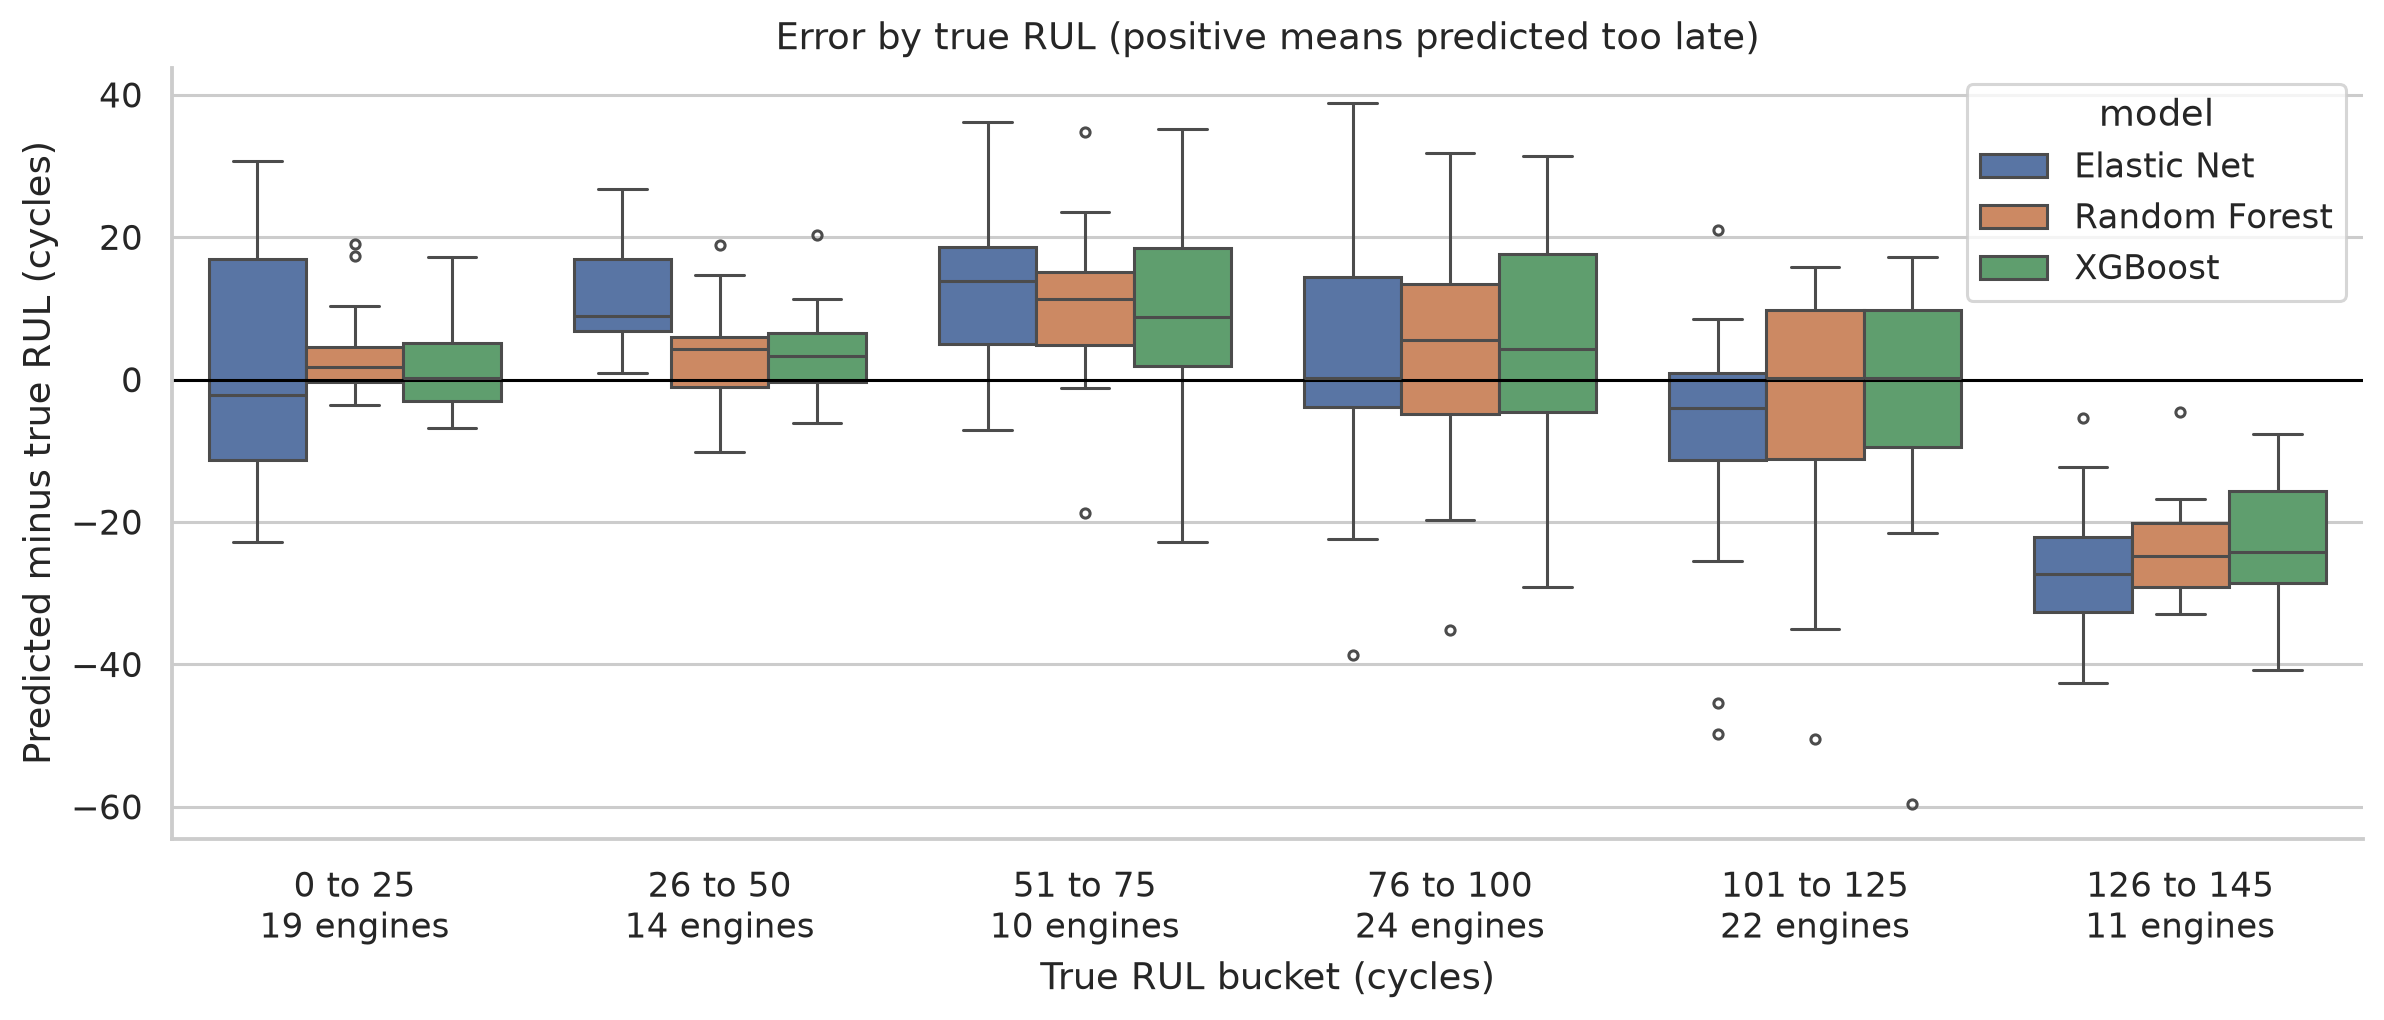
\includegraphics[width=\textwidth]{../figures/results_error_by_bucket.png}
  \caption{Prediction error (predicted minus true RUL) by true RUL bucket for
  the three tuned models on engineered features. Positive errors are late
  predictions.}
  \label{fig:results-buckets}
\end{figure*}

The residual distributions (Fig.~\ref{fig:results-residuals}) are centred
near zero, with mean errors between $-1.0$ and $+0.1$ cycles. The difference
in score between the two ensembles comes from the costly side: 6 Random
Forest predictions and 9 XGBoost predictions are more than 20 cycles late.
Because $S$ grows exponentially with lateness, these few engines account
for most of the gap between 344 and 389, even though the RMSEs are almost
equal.

\begin{figure}[t]
  \centering
  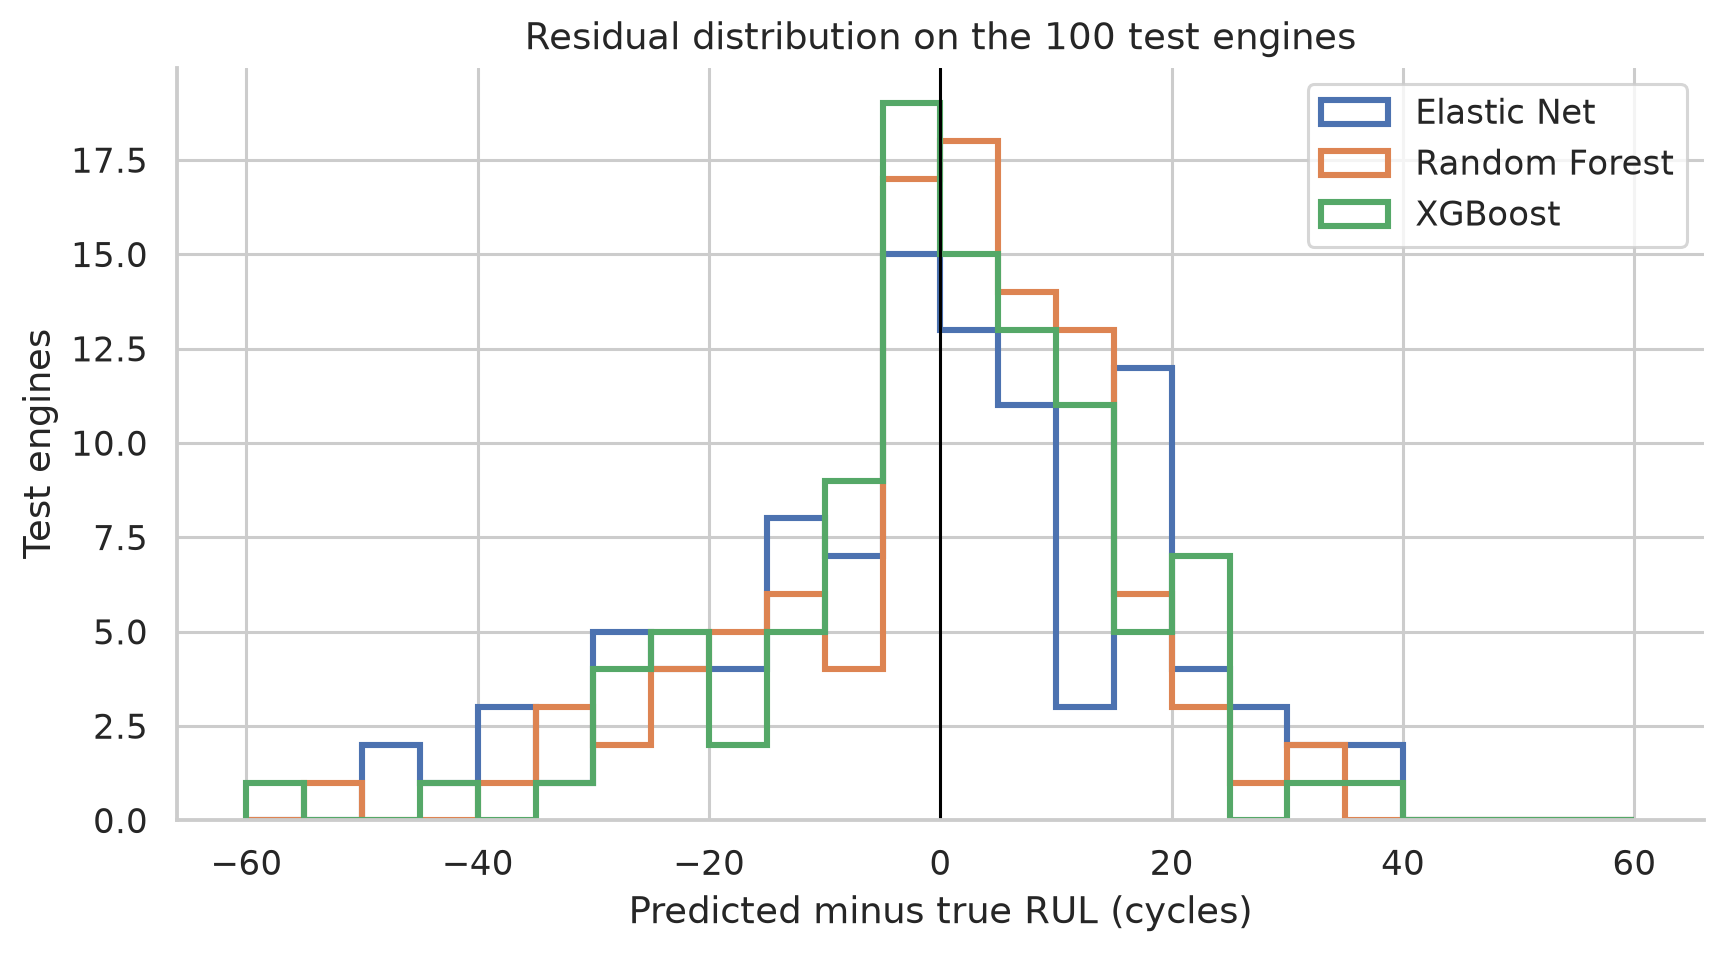
\includegraphics[width=\columnwidth]{../figures/results_residuals.png}
  \caption{Distribution of test errors for the three tuned models on
  engineered features.}
  \label{fig:results-residuals}
\end{figure}

\subsection{Comparison with published results}
Published FD001 results typically train on RUL capped at 125 and score one
prediction per test engine, as we do, but many also clip the test labels at
the cap. For a like for like comparison we rescore our models against the
test RUL clipped at 125. Table~\ref{tab:published} lists every FD001 result
with both RMSE and score collected by Ragab et al.~\cite{ragab2020attention},
except an SVM baseline (RMSE 40.72). By RMSE our Random Forest (14.02) and
XGBoost (14.08) rank fifth and sixth. They improve on the published Random
Forest (17.91) and gradient boosting (15.67) of Zhang et
al.~\cite{zhang2017modbne} and on six deep models, from CNN-LSTM (14.40) to
the 2D CNN of Babu et al.~\cite{babu2016cnn} (18.45). Our own raw feature
models score 16.58 and 16.37 against the same labels, so in our setting most
of the improvement comes from the engineered features rather than the
learner.

Four published deep models are more accurate: the 1D CNN of Li et
al.~\cite{li2018dcnn} (12.61), the attention model of Ragab et
al.~\cite{ragab2020attention} (12.63), HDNN (13.02) and BLCNN (13.18), between
0.8 and 1.4 cycles of RMSE ahead of our Random Forest. On the score $S$ our
position is weaker: six published models score lower than our Random
Forest (310), including BiLSTM-ED and CNN-LSTM, whose RMSE is higher than
ours but whose predictions are less often badly late. The models ahead of
ours learn features from windows of the raw sensor sequence; phase 2 of this
project tests sequence models of this kind. Published protocols differ in
details that are not always reported, such as window length, so differences
of a fraction of a cycle should not be over read.

\begin{table}[t]
\centering
\caption{FD001 test results against labels clipped at 125; ours use the
engineered features. Published values as collected in
\cite{ragab2020attention}, Table III, which cites the original papers for
rows without a reference here.}
\label{tab:published}
\begin{tabular}{lrr}
\hline
Method & RMSE & Score $S$ \\
\hline
1D CNN \cite{li2018dcnn}             & 12.61 & 274 \\
ATS2S \cite{ragab2020attention}      & 12.63 & 243 \\
HDNN                                 & 13.02 & 245 \\
BLCNN                                & 13.18 & 302 \\
Random Forest (ours)                 & 14.02 & 310 \\
XGBoost (ours)                       & 14.08 & 347 \\
CNN-LSTM                             & 14.40 & 290 \\
BiLSTM-ED                            & 14.74 & 273 \\
LSTMBS                               & 14.89 & 481 \\
MODBNE \cite{zhang2017modbne}        & 15.04 & 334 \\
Gradient boosting \cite{zhang2017modbne} & 15.67 & 474 \\
Deep LSTM \cite{zheng2017lstm}       & 16.14 & 338 \\
Elastic Net (ours)                   & 17.01 & 469 \\
Random Forest \cite{zhang2017modbne} & 17.91 & 480 \\
2D CNN \cite{babu2016cnn}            & 18.45 & 1287 \\
\hline
\end{tabular}
\end{table}

% ABOUTME: Discussion and limitations section of the IEEE report.
% ABOUTME: Interprets the cross validation, test and explainability results and states the limits of the study.
\section{Discussion and Limitations}
\label{sec:discussion}

\subsection{Features and learners}
Both the feature set and the model family matter. Against the true test
labels, engineered features lower the RMSE by 2.22 cycles for XGBoost,
2.54 for Random Forest and 4.30 for Elastic Net, while replacing Elastic
Net with XGBoost lowers it by 4.99 on raw features and 2.91 on engineered
features; cross validation shows the same pattern. The paired bootstrap
interval for XGBoost on engineered minus raw features ($-4.4$ to $-0.2$
cycles) excludes zero, while the interval for Random Forest minus XGBoost
($-1.3$ to $+1.1$) does not, so once the features are fixed the choice
between the two tree ensembles makes no measurable difference on 100 test
engines. Our margin over the published Random Forest~\cite{zhang2017modbne}
comes mainly from the features: against labels clipped at 125 our Random
Forest scores 16.58 on raw sensors and 14.02 on engineered features,
against 17.91 published. The ablation of
Section~\ref{sec:features} places most of the feature gain on the rolling
slopes, which give the rate of degradation rather than its level.

\subsection{Accurate near failure, coarse far from it}
Both ensembles are accurate where maintenance is decided. On the 33 test
engines with true RUL of at most 50 cycles, the late-stage RMSE is 7.34
for Random Forest and 7.03 for XGBoost, against 17.88 and 18.11 on the 67
early-stage engines. Part of the early-stage error is built into the
target: eleven test engines have a true RUL above the training cap, and
no model on engineered features predicts above 130, so these engines are underestimated by
construction. This error only brings maintenance forward. The costlier
error appears between 51 and 75 cycles, where all three models predict too
late (median error $+9$ to $+14$ cycles), around the point at which
degradation first becomes visible in the sensors. Late predictions are the
error that the score $S$ penalises most.

\subsection{Model selection and the test set}
Cross validation selected XGBoost (RMSE 13.99 against 14.42 for Random
Forest), while Random Forest is marginally better on the test set (RMSE
15.23 against 15.36, score 344 against 389). We kept the selection made
before the test set was opened. The bootstrap interval above shows that the
test ranking of the two ensembles is within sampling noise, and most of the
score gap comes from a single engine that XGBoost predicts about 9 cycles
earlier than Random Forest (Section~\ref{sec:results}). Cross validation and test numbers are not
directly comparable: cross validation scores every cycle against the
capped target, whereas the test set scores one cycle per engine against
the true RUL. The cross validation scores of the selected configurations
are also optimistic, because the same folds chose and scored them.

\subsection{What the models rely on}
Held-out permutation importance shows that both ensembles depend mainly on
two inputs: the health index, whose shuffling raises RMSE by about 11
cycles for XGBoost and 7.4 for Random Forest, and the cycle number (4.84
and 5.22). No individual sensor group adds more than 1.62. The sensor
information therefore reaches the models largely through the health index,
a single learned combination of all 14 sensors. Reliance on the cycle
number means the models partly predict from age. This is useful on FD001,
where every engine starts in normal condition and training lifetimes span
128 to 362 cycles, but it ties the models to the lifetime distribution of
this fleet. Impurity and permutation importance also disagree for
correlated inputs: \texttt{s\_4} receives 26\% of Random Forest's impurity
reduction but costs only 1.62 cycles when shuffled, so impurity rankings
alone would overstate its role.

\subsection{Gap to deep sequence models}
Four published deep models are more accurate than our Random Forest and
XGBoost by 0.8 to 1.5 cycles of RMSE against clipped labels, and on the
score $S$ six published models do better than our Random Forest and eight
better than the selected XGBoost. These models learn
features from windows of the raw sensor sequence. Our features look back
at most 20 cycles and use window lengths chosen by hand, so they cannot
represent how long a sensor has been drifting or when its drift began to
accelerate. The remaining gap is consistent with this limit, although our
experiments do not isolate it.

\subsection{Limitations}
All results are on FD001, which has a single operating condition and a
single fault mode. The regime normalisation of Section~\ref{sec:features}
reduces to a z-score here and has not been tested on the multi-condition
subsets. The test set has 100 engines with one prediction each, so the
test metrics carry wide sampling intervals, as the bootstrap shows; the
late stage contains only 33 engines. The cap of 125 cycles bounds what the
models can predict, so engines with more remaining life are always
underestimated. Published FD001 results differ in protocol details that
are not always reported, such as whether test labels are clipped and the
window length used, so the comparison with them is approximate. Finally,
C-MAPSS is simulated, and conclusions about which sensors matter apply to
the simulation rather than to physical engines.

% ABOUTME: Conclusion section of the IEEE report.
% ABOUTME: Summary of Phase 1 findings and the plan for sequence models in Phase 2.
\section{Conclusion and Phase 2 Plan}
\label{sec:conclusion}

We predicted the remaining useful life of FD001 engines with engineered
degradation features and three classical regressors, under a protocol that
splits by engine, refits feature statistics inside every fold and scores
the test set once. The selected XGBoost model reaches a test RMSE of 15.36
cycles overall and 7.03 cycles on engines within 50 cycles of failure.
Against labels clipped at 125, Random Forest and XGBoost reach 14.02 and
14.08, ahead of published Random Forest and gradient boosting results and
0.8 to 1.4 cycles behind the best published deep models. The engineered
features and the tree ensembles both improve on the linear models with raw
sensors, the two tree ensembles cannot be separated on the test set, and
both rely mainly on the health index and the cycle number.

Phase 2 replaces the fixed 20-cycle summaries with models that read the
sensor sequence directly: an LSTM, a temporal convolutional network or a
Transformer encoder on fixed-length windows of the raw sensors. It adds an
ablation study and a hybrid model that feeds the engineered features into
the sequence model, which tests whether the hand-made features still help
once the history is learned. The sequence models will be evaluated under
the protocol of this report: FD001, five-fold cross validation grouped by
engine, training RUL capped at 125, one prediction per test engine scored
once, and the same RMSE, score $S$ and early and late stage metrics, so
that their results are directly comparable with Table~\ref{tab:test-results}.

% ABOUTME: Contributions section of the IEEE report: who did what.
% ABOUTME: One entry per member, with the sections each one wrote.
\section{Contributions}
\label{sec:contributions}

\begin{itemize}
\item \textbf{Sarvesh Srinath}: repository setup, working conventions,
pinned dependencies, continuous integration and the pipeline that reruns
every notebook; the engine-level split and evaluation metrics; the final
test-set evaluation, error analysis and comparison with published results;
reproducibility checks; review and merging of pull requests. Wrote
Sections~\ref{sec:evaluation} and~\ref{sec:results}.
\item \textbf{Trishit Swarnakar}: loading of FD001 and construction of the
RUL target; exploratory data analysis, sensor selection and the choice of
target cap. Wrote Section~\ref{sec:data}.
\item \textbf{Aryan Kumar}: degradation feature engineering (regime
normalisation, rolling statistics, rolling slopes and health index) and the
feature ablation. Wrote Section~\ref{sec:features}.
\item \textbf{Husain Khorakiwala}: model implementation, baselines and
hyperparameter tuning with engine-grouped cross validation; the RUL cap
experiment; feature importance and SHAP analysis; review of the test-set
evaluation and reproducibility work. Wrote Section~\ref{sec:models}.
\item \textbf{Navodit Sharma}: literature review; assembly of the report;
presentation slides.
Wrote the abstract and Sections~\ref{sec:intro}, \ref{sec:related},
\ref{sec:discussion} and~\ref{sec:conclusion}.
\end{itemize}


\bibliographystyle{IEEEtran}
\bibliography{refs}

\end{document}
